\documentclass[oneside,final]{report}

\usepackage{graphicx}
\usepackage[parfill]{parskip}
\usepackage[section] {placeins}

\graphicspath{{images/}}

\begin{document}
 

% ================ Front Matter ================
% Suppress page number for title page and letter of submittal
\pagestyle{empty}

% ==== Title Page
\begin{flushright}
 \begin{LARGE}
  \textbf{UNIVERSITY OF WATERLOO}
 \end{LARGE}

 \begin{large}
  Faculaty of Mechatronics Engineering\\[4cm]
 \end{large}

 \begin{LARGE}
  \textbf{
    Fourth Year Design Project \\[0.0cm]
    Final Design Report
  }
 \end{LARGE}

 \vfill

  Prepared By: \\[0.2cm]
  Iain Peet - 20252201\\
  Jordan Valentin - 20271260\\
  Rowan Head-Marsden - 20271527\\
  \today
\end{flushright}
\clearpage

% ==== Letter of Transmittal
\today \\[0.5cm]

Faculty of Mechatronics Engineering \\
University of Waterloo \\
Waterloo, Ontario \\

To Whom It May Concern:

Lorem ipsum dolor est... \\[0.5cm]

Sincerely, \\[1cm]

Iain Peet \hspace{4cm} Jordan Valentin \hspace{4cm} Rowan Head-Marsden
\clearpage

% Resume page numbering
\pagestyle{plain}
\setcounter{page}{1}
\pagenumbering{roman}

% ==== Table of Contents
\tableofcontents

% ==== List of Figures
\listoffigures
\addcontentsline{toc}{chapter}{List of Tables and Figures}

\chapter*{Executive Summary}
\addcontentsline{toc}{chapter}{Summary}

% ====================== Report Body =================================
\clearpage
\setcounter{page}{1}
\pagenumbering{arabic}
\pagestyle{headings}

\chapter{Introduction}

\section{Background}
Powered wheelchairs have obvious benefits for the mobility of the physically disabled.  As relatively heavy, powered vehicles, operation of these wheelchairs also carries obvious risk.  Thus, operators must be capable of safe operations.

Irene Ruel, a physiotherapist in the employ of the British Columbia Interior Health Authority, who has previously been responsible for powered wheelchair assessments in an extended care facilities, was consulted regarding this problem.  By her account, the risk that powered wheelchair operators will collide with other patients is a serious concern, which frequently results in the denial of requests for powered wheelchairs.

\section{Need Statement}
Access to powered wheelchairs may be restricted due to concerns about a patient's capability for safe operation.

Powered wheelchairs can improve the mobility of the physically handicapped, but alertness and control are required for safe operation.  Additional assistive technology is needed in order to afford the same benefits to the more severely disabled.

\section{Objectives and Constraints}
The objectives of this design problem are as follows:

\begin{itemize}
 \item \emph{Improve safety}.  Safety is a significant concern for powered wheelchair operation.  Effective safety systems will be of great value to those with physical disabilities.
 \item \emph{Improve accessibility}.  For those who would be denied access to a powered wheelchair, a safety system which permits access will have significant quality-of-life benefits.
 \item \emph{Assist with difficult tasks}. Some tasks, such as precise positioning and movement in constrained spaces, are difficult even for unimpaired operators.   A system which can assist with such tasks would be helpful.
\end{itemize}

The constraints of the design are as follows:

\begin{itemize}
 \item \emph{Insensitive to operating environment}.  Realistic operating environments will be varied, and subject to change.  The usefulness of a safety system will be severely degraded if it depends on a specialized, controlled environment.
 \item \emph{Integrates with existing wheelchairs}.  Powered wheelchairs are expensive, and many are already in existence.  The potential reach of a new safety system will be severely restricted if it may not be integrated with pre-existing wheelchairs.
 \item \emph{Cost kept below \$500}.  The system will be paid for by end users, who will be sensitive to cost.  It will be difficult to market a system which is very expensive relative to the cost of a basic powered wheelchair.
\end{itemize}

\section{Criteria}
\begin{figure}[hbt]
 \centering
 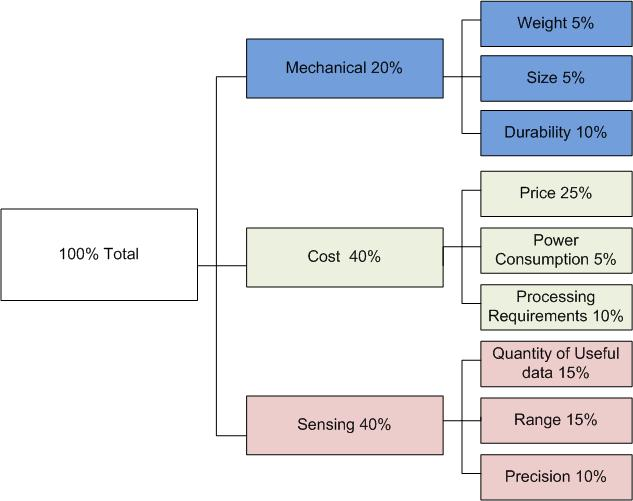
\includegraphics[scale=0.5]{CriteriaWeighting}
 \caption{Criteria Weighting} \label{fig:criteria_weighting}
\end{figure}

\subsection{Weight}
Weight is an important criterion as a number of powered wheel chairs have weight limitations. This should be as small as possible since the weight capacity of a chair like the Invacare Neutron R51LXP is 300 pounds \cite{wheelchair_data}. This means that for any weight we add on to the wheel chair we reduce the potential carrying load of the wheel chair and with it our potential market.

\subsection{Size}
Size is a minor criterion we considered, with an excessively large bulky attachment it would reduce the mobility of the wheel chair and decrease the number of places the wheel chair can travel to. It may also get in the way of the user when operating the wheel chair. This made it important to have some size criteria for measuring the strength of a design.

\subsection{Durability}
While most of the system should not be placed under continuous strain or be at high risk of damage, it is important to consider how durable the design is as there will be wear and tear from use of this system on a wheel chair and damage occurred from movement around the wheel chair.

\subsection{Price}
Price is an important factor for our consideration since we plan to market it to the end users and not to corporations that may have larger budgets. This then made it the most important ranking and with the very large difference in sensor costs it made for a very important factor in determining which route to take.

\subsection{Power Consumption}
Power Consumption measure how much an addition will add to the power consumption of the wheel chair. Many of these chairs are run off of an onboard battery and draining this battery quickly will significantly reduce its usefulness to the users. 

\subsection{Processing Requirements}
The amount of computational intelligence required to handle the data that is coming in from the sensor. This is to make distinction between sensors similar to a Kinect which uses USB and would be plugged into a lab top that will be needed to interpret the data versus something like a sonar sensor that could be tuned and used on FPGA. This will run opposite the Quantity of Useful Data.

\subsection{Quantity of useful Data}
This was selected to distinguish things like sonar which provide simply a distance mapping for a cone versus something like the lydar that provides a depth map using a large number of points. The more data we get from a sensor the more we can make use of it to recognize and avoid obstacles. This runs as the opposite of processing requirements, since more data requires more processing power to interpret the data.

\subsection{Range}
The range for the detection of objects is fairly important to us. While range beyond 7-8 meters is not particularly useful, we want range from about 0 to 8 meters optimally. For this we assume they are working in optimal conditions which we said to be indoors and with normal lighting. Certain sensors we consider have significantly reduced range in other conditions.

\subsection{Precision}
Precision is fairly important since we are detecting obstacles and we would like to know how far away they are, noise and disturbances are acceptable to a small degree so long as we can identify them as noise and not a fast moving obstacle. In addition to this it’s important that some sensors have decreased precision at increased range. This is noted as a small reduction in their score.

\section{Patents}
% TODO(jordan)


\chapter{Proposed Solution}

\section{Mechanical Designs}
\subsection{Design \#1}
\begin{figure}[hbt]
 \centering
 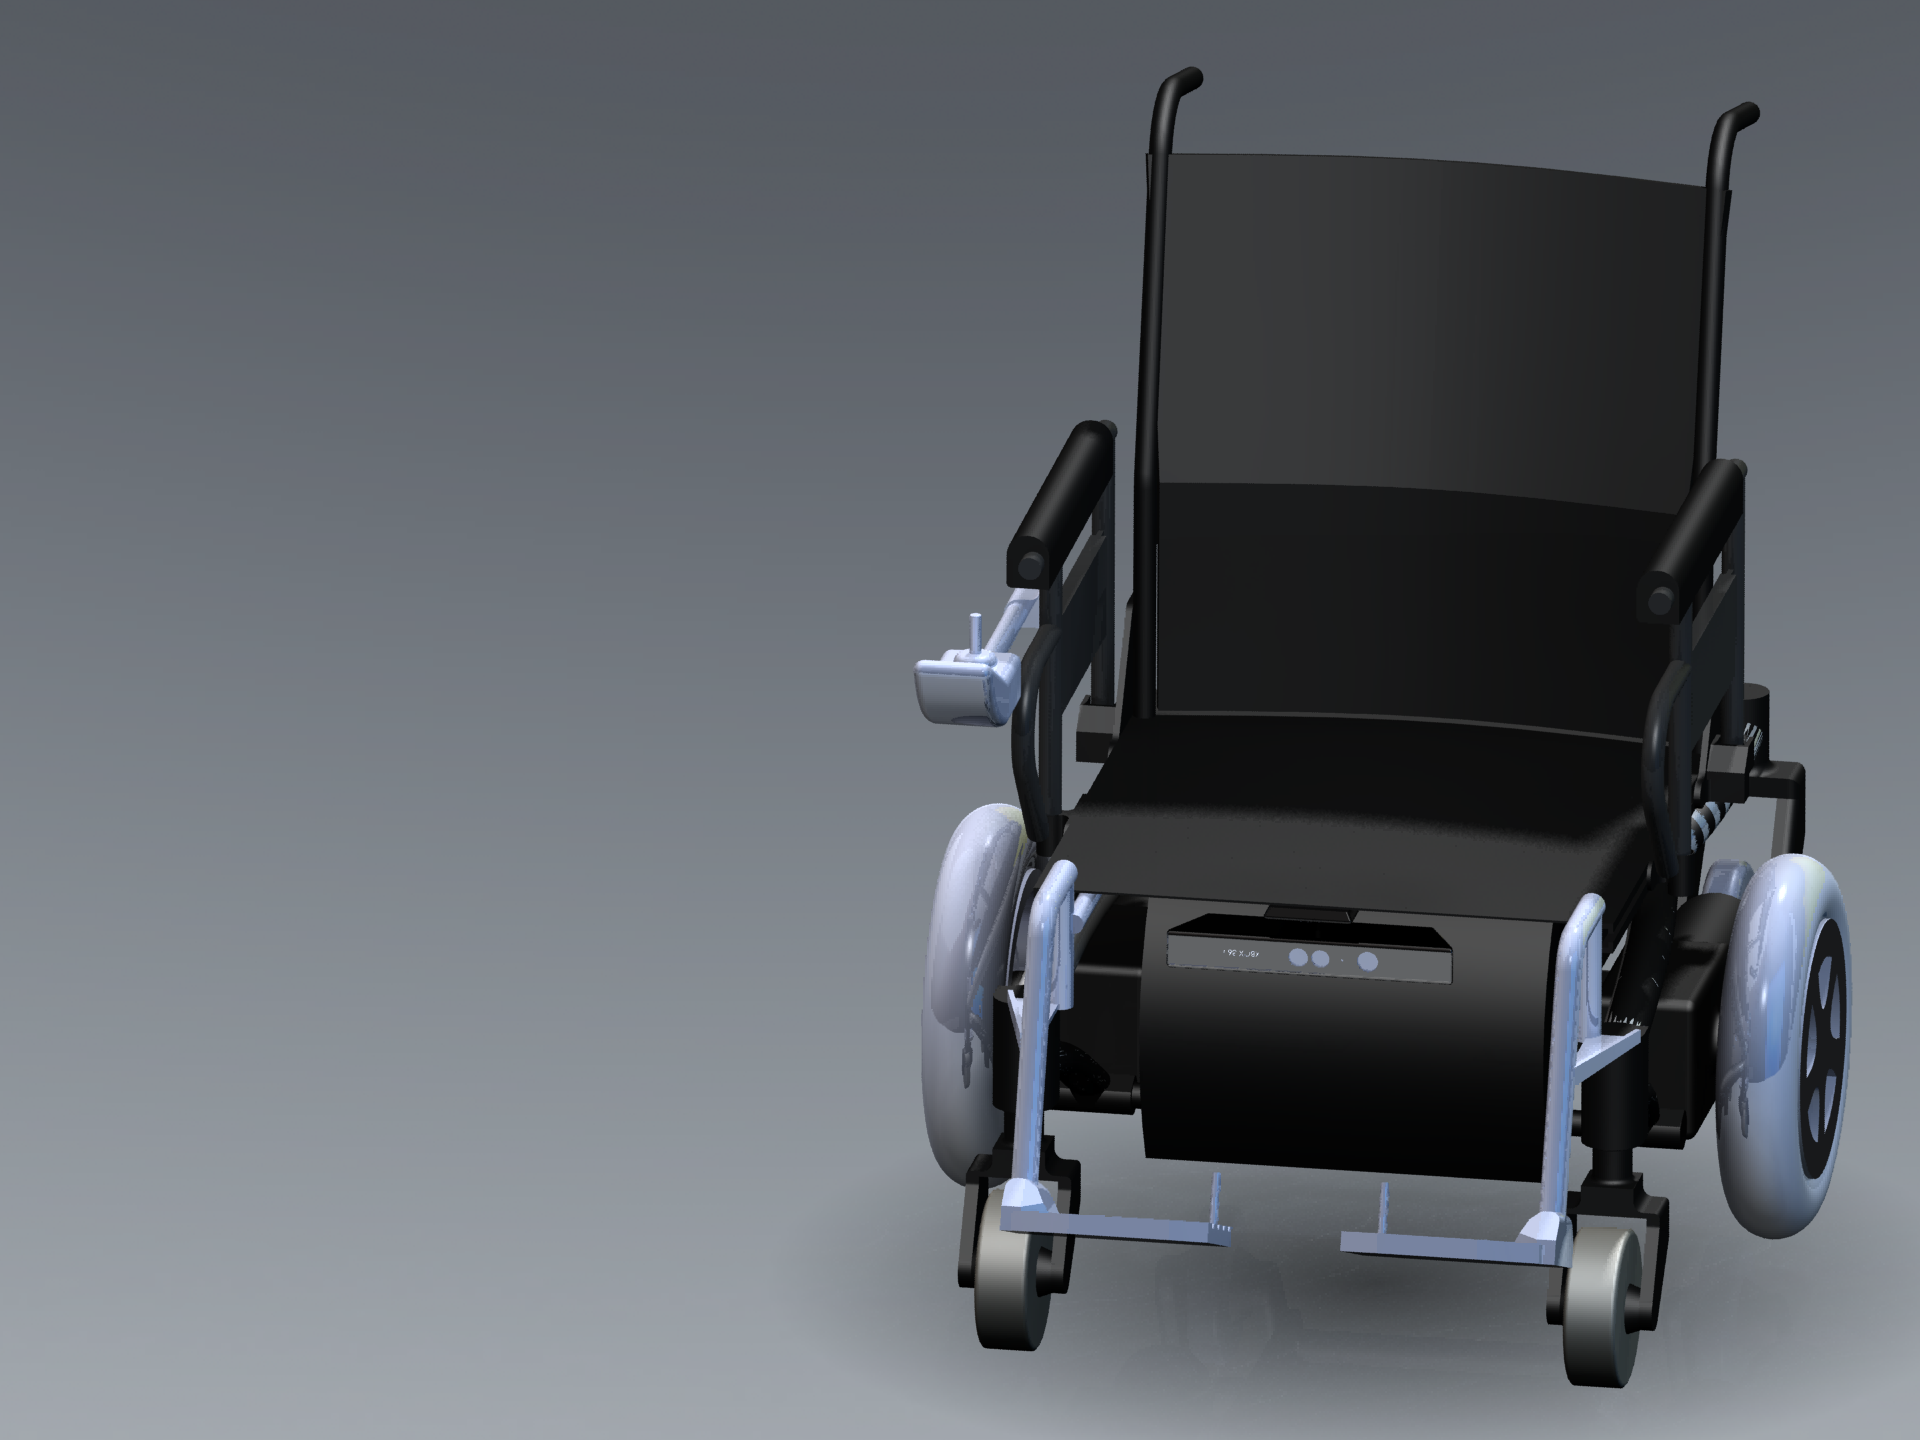
\includegraphics[scale=0.15]{WheelChair_1}
 \caption{Wheelchair Design \#1}
\end{figure}

One option was to mount the Kinect up above the user so that the user could sit in the chair with no impedances. The sensor would then have a forward looking vision viewing overtop of the user sitting in the seat. This design had the advantages of being easy to implement and much similar to the approach taken with manpowered wheel chairs with a second person pushing the chair in the appropriate direction. In addition to this the design has no inconveniences for the user since everything is mounted outside of a region where they mount or dismount. In addition to that it maintains the ability for the arms to be pushed backwards so that the user can exit via the side of the wheel chair for movements like switching from a wheel chair on to a bed or toilet.

The main disadvantage of this mounting form is that the Kinect needs to be mounted about 1m above the seat in order to meet the 95th percentile marker for males. This means that the data taken from the Kinect will need to have a transform applied to it in order to be useful to the users. Another added disadvantage is that with the Kinect mounted 1m up we add 1 m to the distance the Kinect sees all obstacles at. This is a significant reduction of the Kinects range and with it there is a reduction in the Kinects precision. One final thing is that parts of the image need to be ignored in this configuration since the Kinect cant be allowed to interpret the user as an obstacle. The 95th percentile length for the legs is that they will stick out 55 cm from the buttocks \cite{NASA}. This means that there will be a fair bit of lost data and very close proximity obstacles will be invisible to the sensor.

\subsection{Design \#2}
\begin{figure}[hbt]
 \centering
 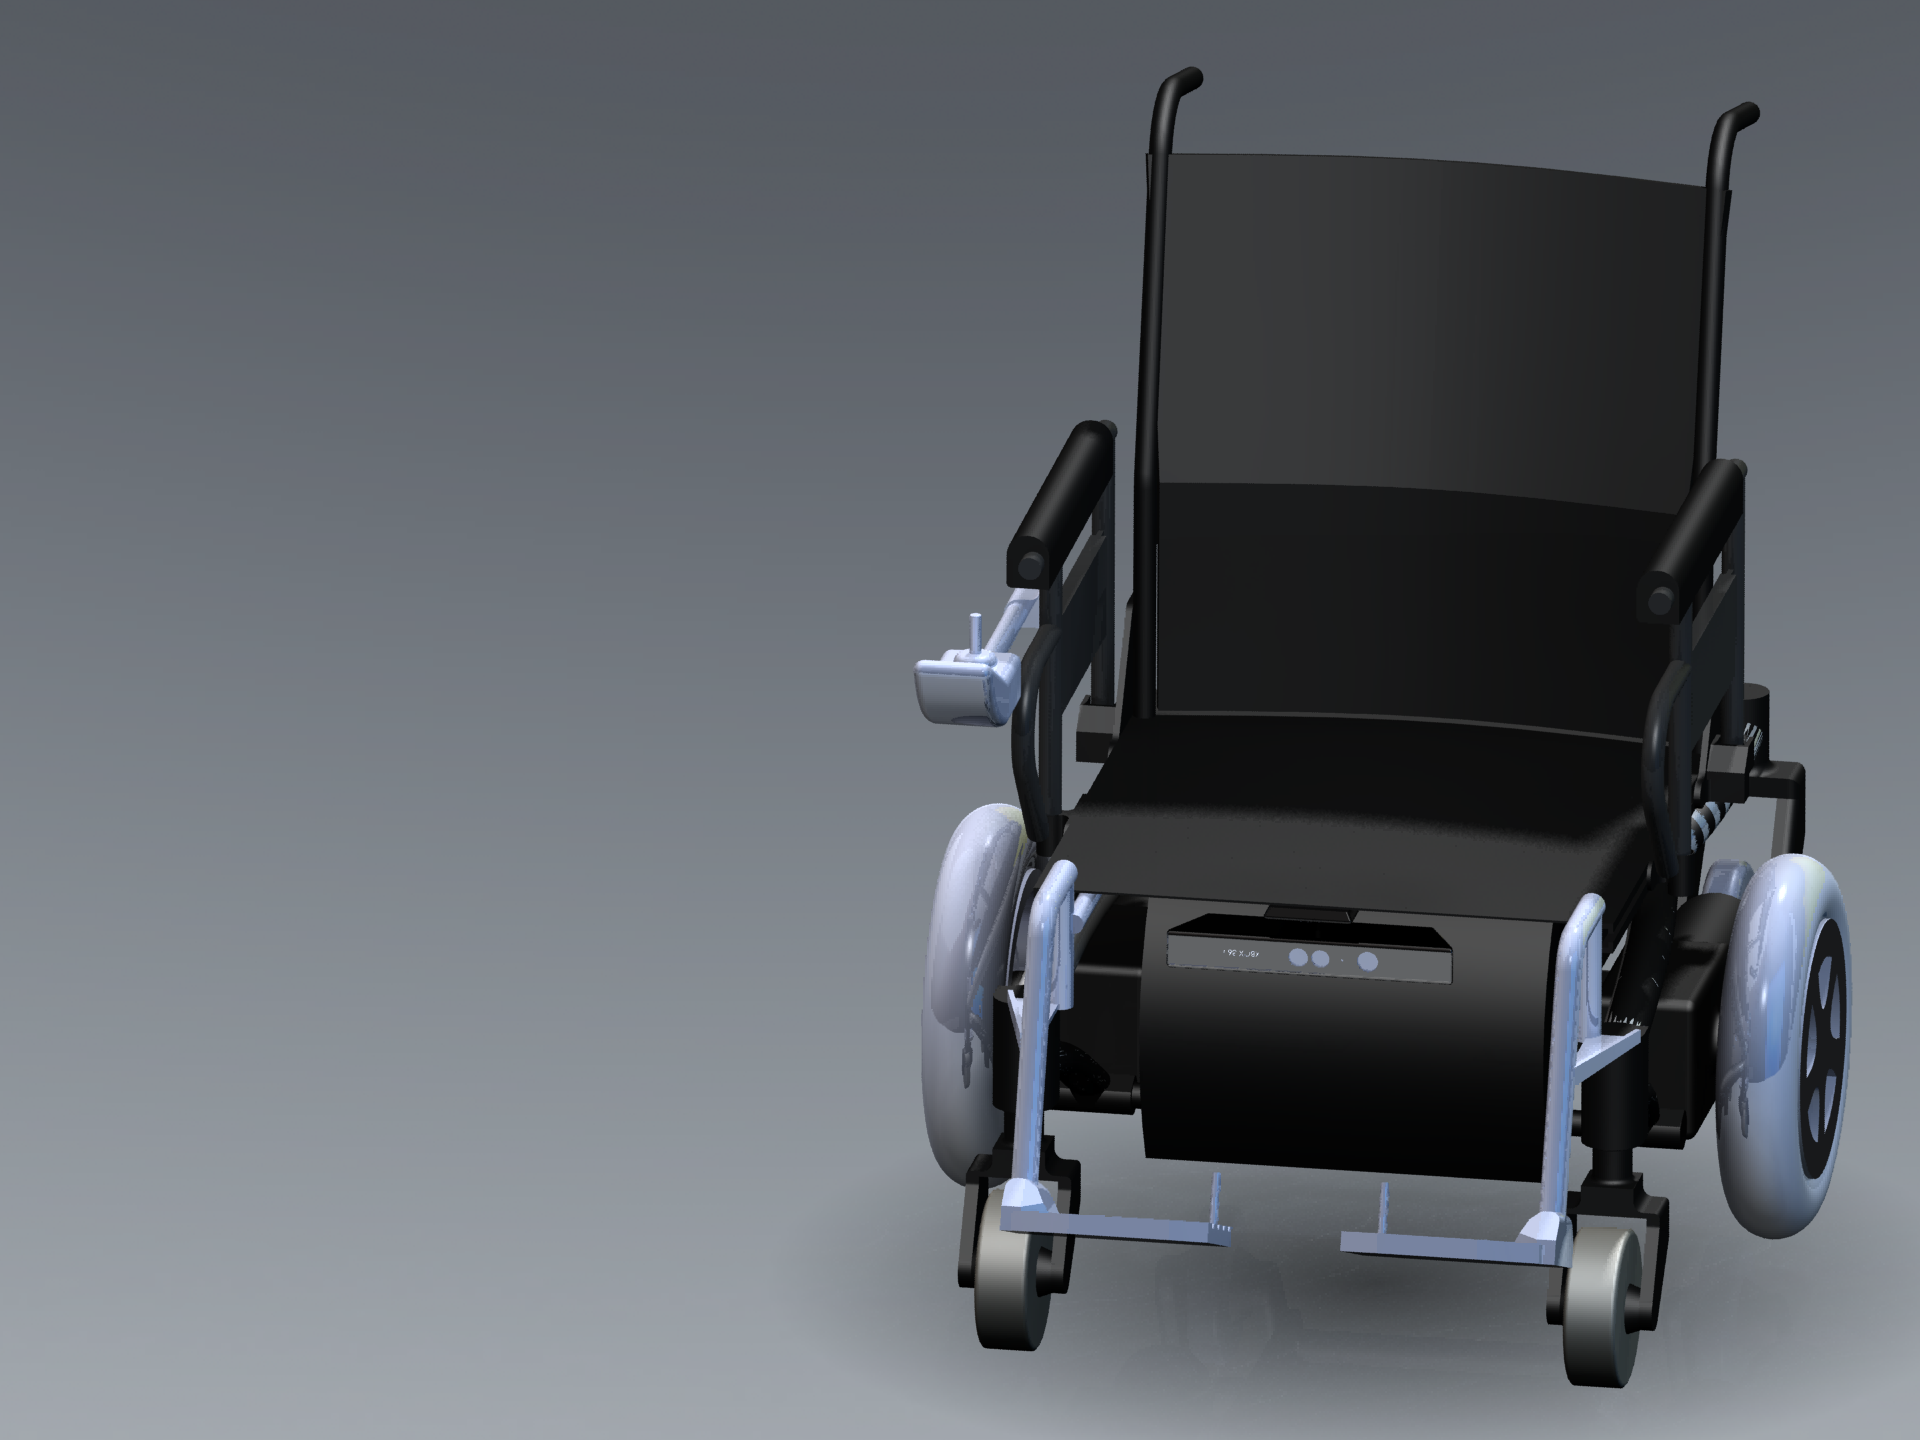
\includegraphics[scale=0.15]{WheelChair_2}
 \caption{Wheelchair Design \#2}
\end{figure}

The second design idea was to place the Kinect sensor on the bottom of the chair.  This had the advantages of being placed out of the way so the Kinect was still not in the way of the user however it places the Kinect at the same level as we would like it for sensing obstacles.It also has the advantage of being very close to the front of the chair providing the best range and precision. Lastly it also maintains the freedom of mobility that the user has with respect to pulling up the arms and exiting to a side.

The disadvantage to this is that when a user sits in the chair they often place their legs in such a way that they block the vision of the Kinect. This would effectively make all the sensors blind when the user sits in a specific orientation. Since we can’t allow this, the design was ruled out as a possible solution for where to place the Kinect sensor.

\subsection{Design \#3}
\begin{figure}[hbt]
 \centering
 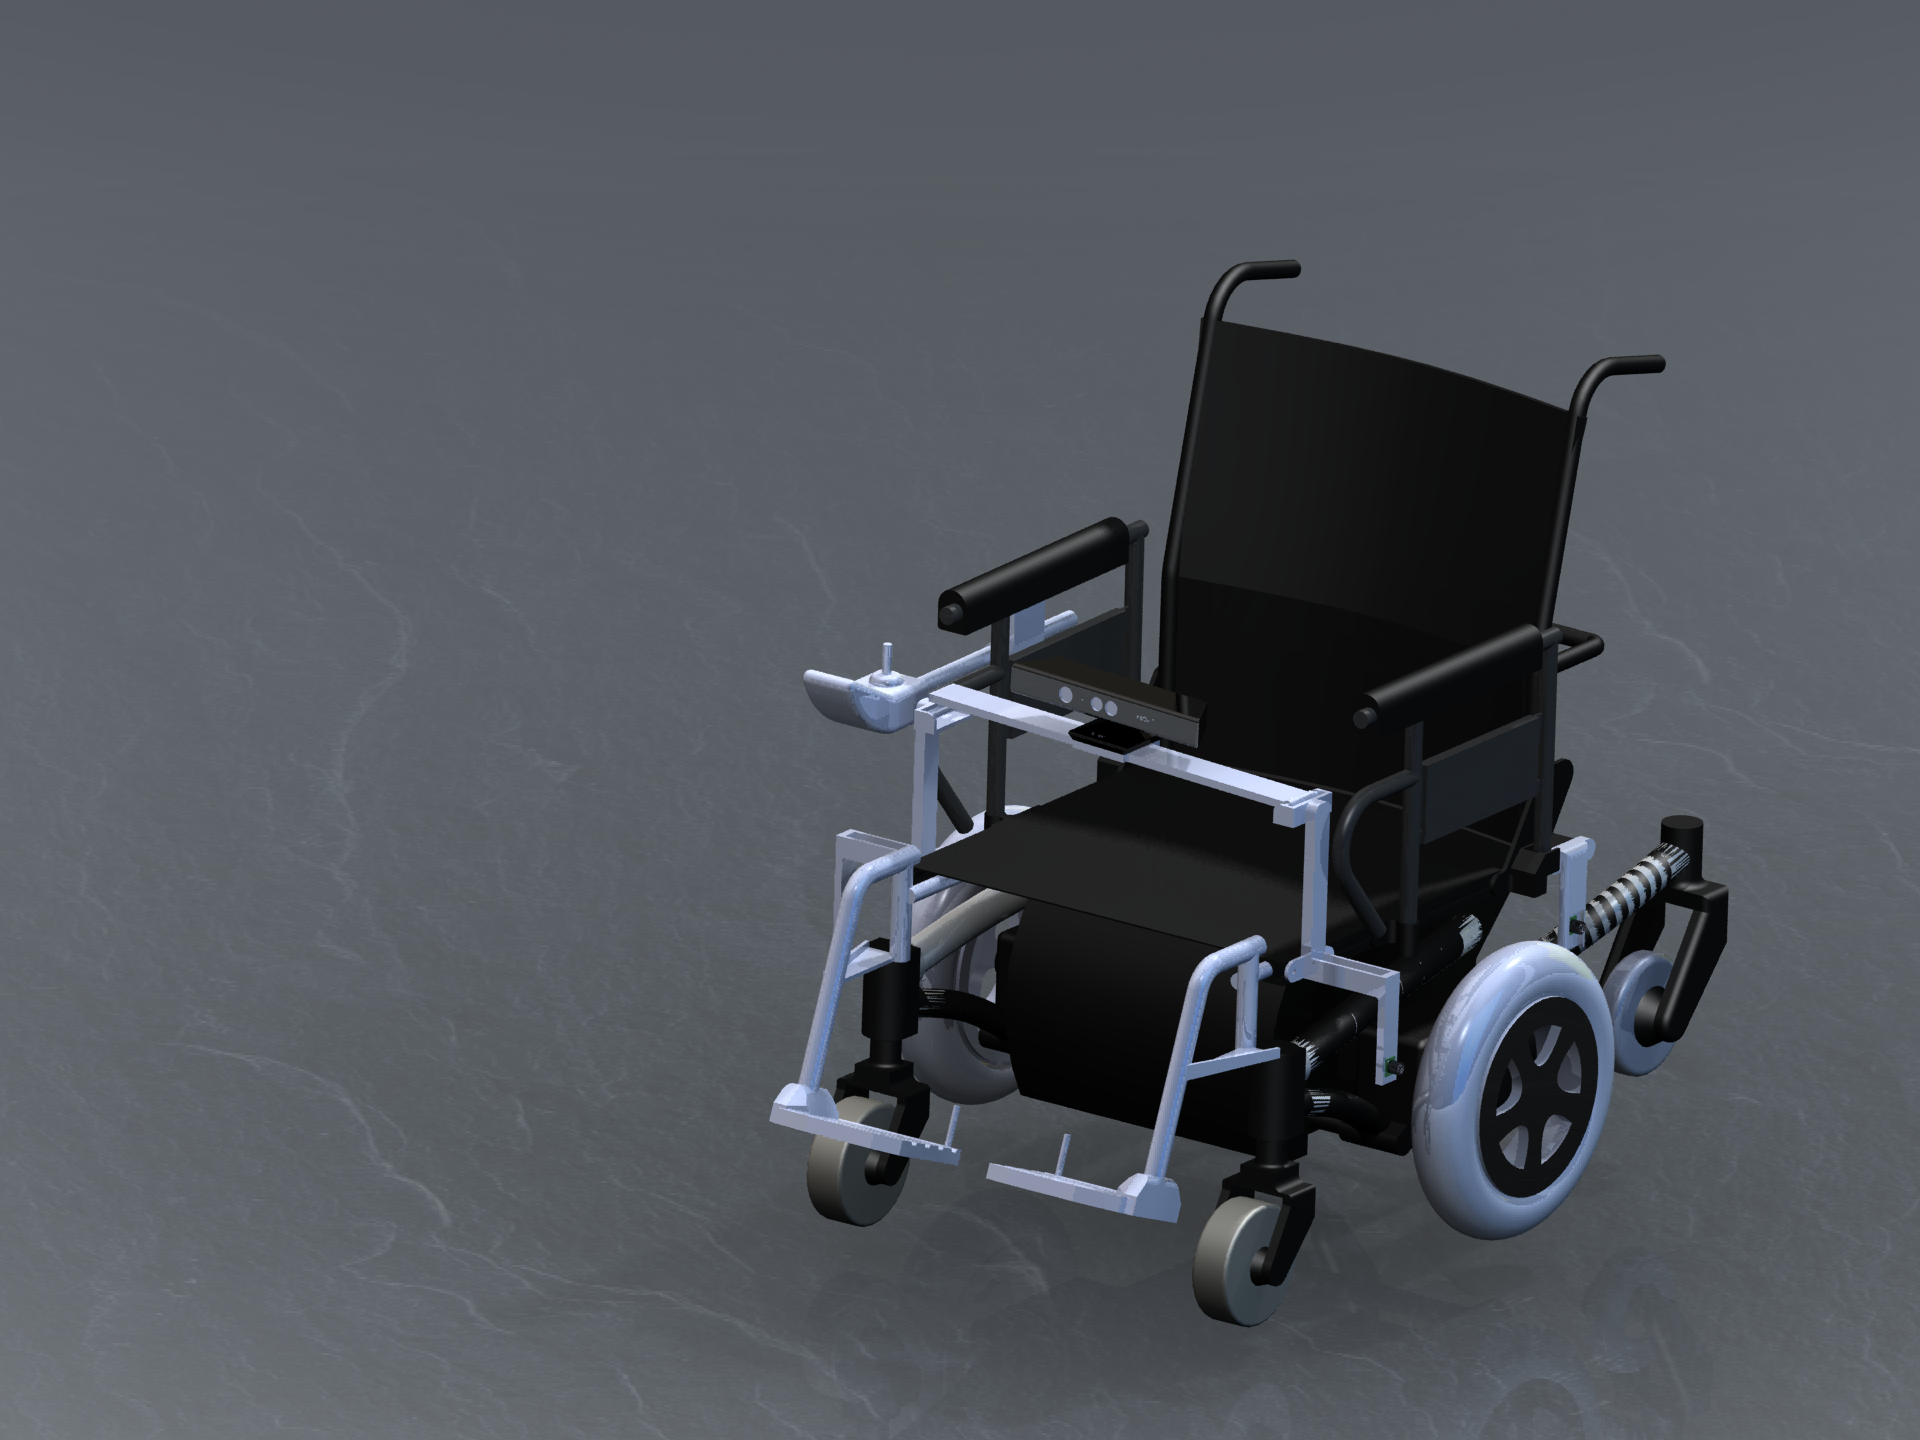
\includegraphics[scale=0.15]{WheelChair_Final}
 \caption{Wheelchair Design \#3}
\end{figure}

Our final design made use of a concept similar to the trays found on airplanes or trains. The folding table can be lowered into position with the mounted Kinect on top of it. This has the advantage of no interference with the sensor, with it mounted at the front of the chair it makes optimal use of range and precision of the Kinect. With the sensor roughly on level with what we need it is possible to consider the occupancy map generated by the Kinect without needing to perform any transforms to get the correct orientation.

The disadvantages to this are that it is moderately more complicated mechanically since the Kinect mounting needs to be designed and made separately. There are also minor inconveniences to the user when they are attempting to get into or out of the wheel chair. It does not allow the user to move out of the chair via one of the other two sides to the chair the way the other designs do. 


\section{Mechanical Design Selection}
% TODO(rowan)

\section{Sensor Selection}

Using the criteria mentioned earlier in the report along with their respective weightings, a decision-making matrix was formed and is shown in Table \ref{tab:decision_matrix}.

    \begin{table}[hbt]
        \caption{Decision Making Matrix}
        \centering
        \begin{tabular}{cc}
        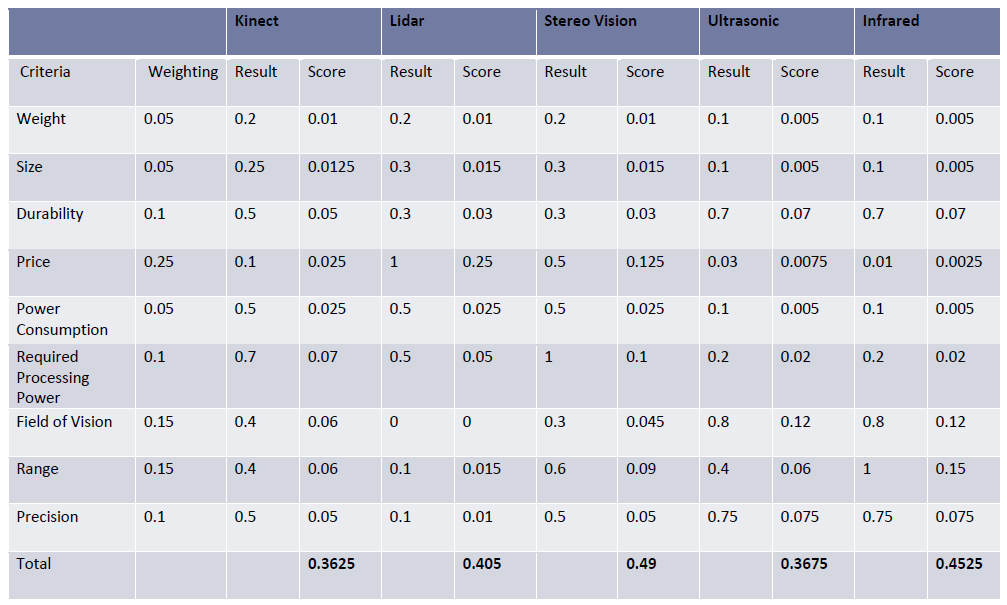
\includegraphics[scale=0.35]{decision_matrix}\\
        \end{tabular}
        \label{tab:decision_matrix}
    \end{table}

The decision making matrix shows the best sensors according to the projects criteria and weightings, as seen in Table \ref{tab:decision_matrix}. The lowest value was the best in this case since for a number of the criteria lower values represented a better performance such as cost, weight, size, power consumption. This means that the best two sensors were the Xbox Kinect and Sonar. 

These sensors are close in weighting, but operate very differently in practice. The Kinect gives a very large amount of data, both range and bearing, about its field of view. The sonar sensors give less information but are quite cheap. The final solution, since these sensors are weighted so closely, was to use a combination of the two sensors. The Kinect provides accurate and resonably precision data in the direction of movement of the chair, and the sonar sensors provide more coarse collision data about the periphery to prevent collisions from the side.

\chapter{Detailed Design}

\section{System-Level Design}
\begin{figure}[hbt]
 \centering
 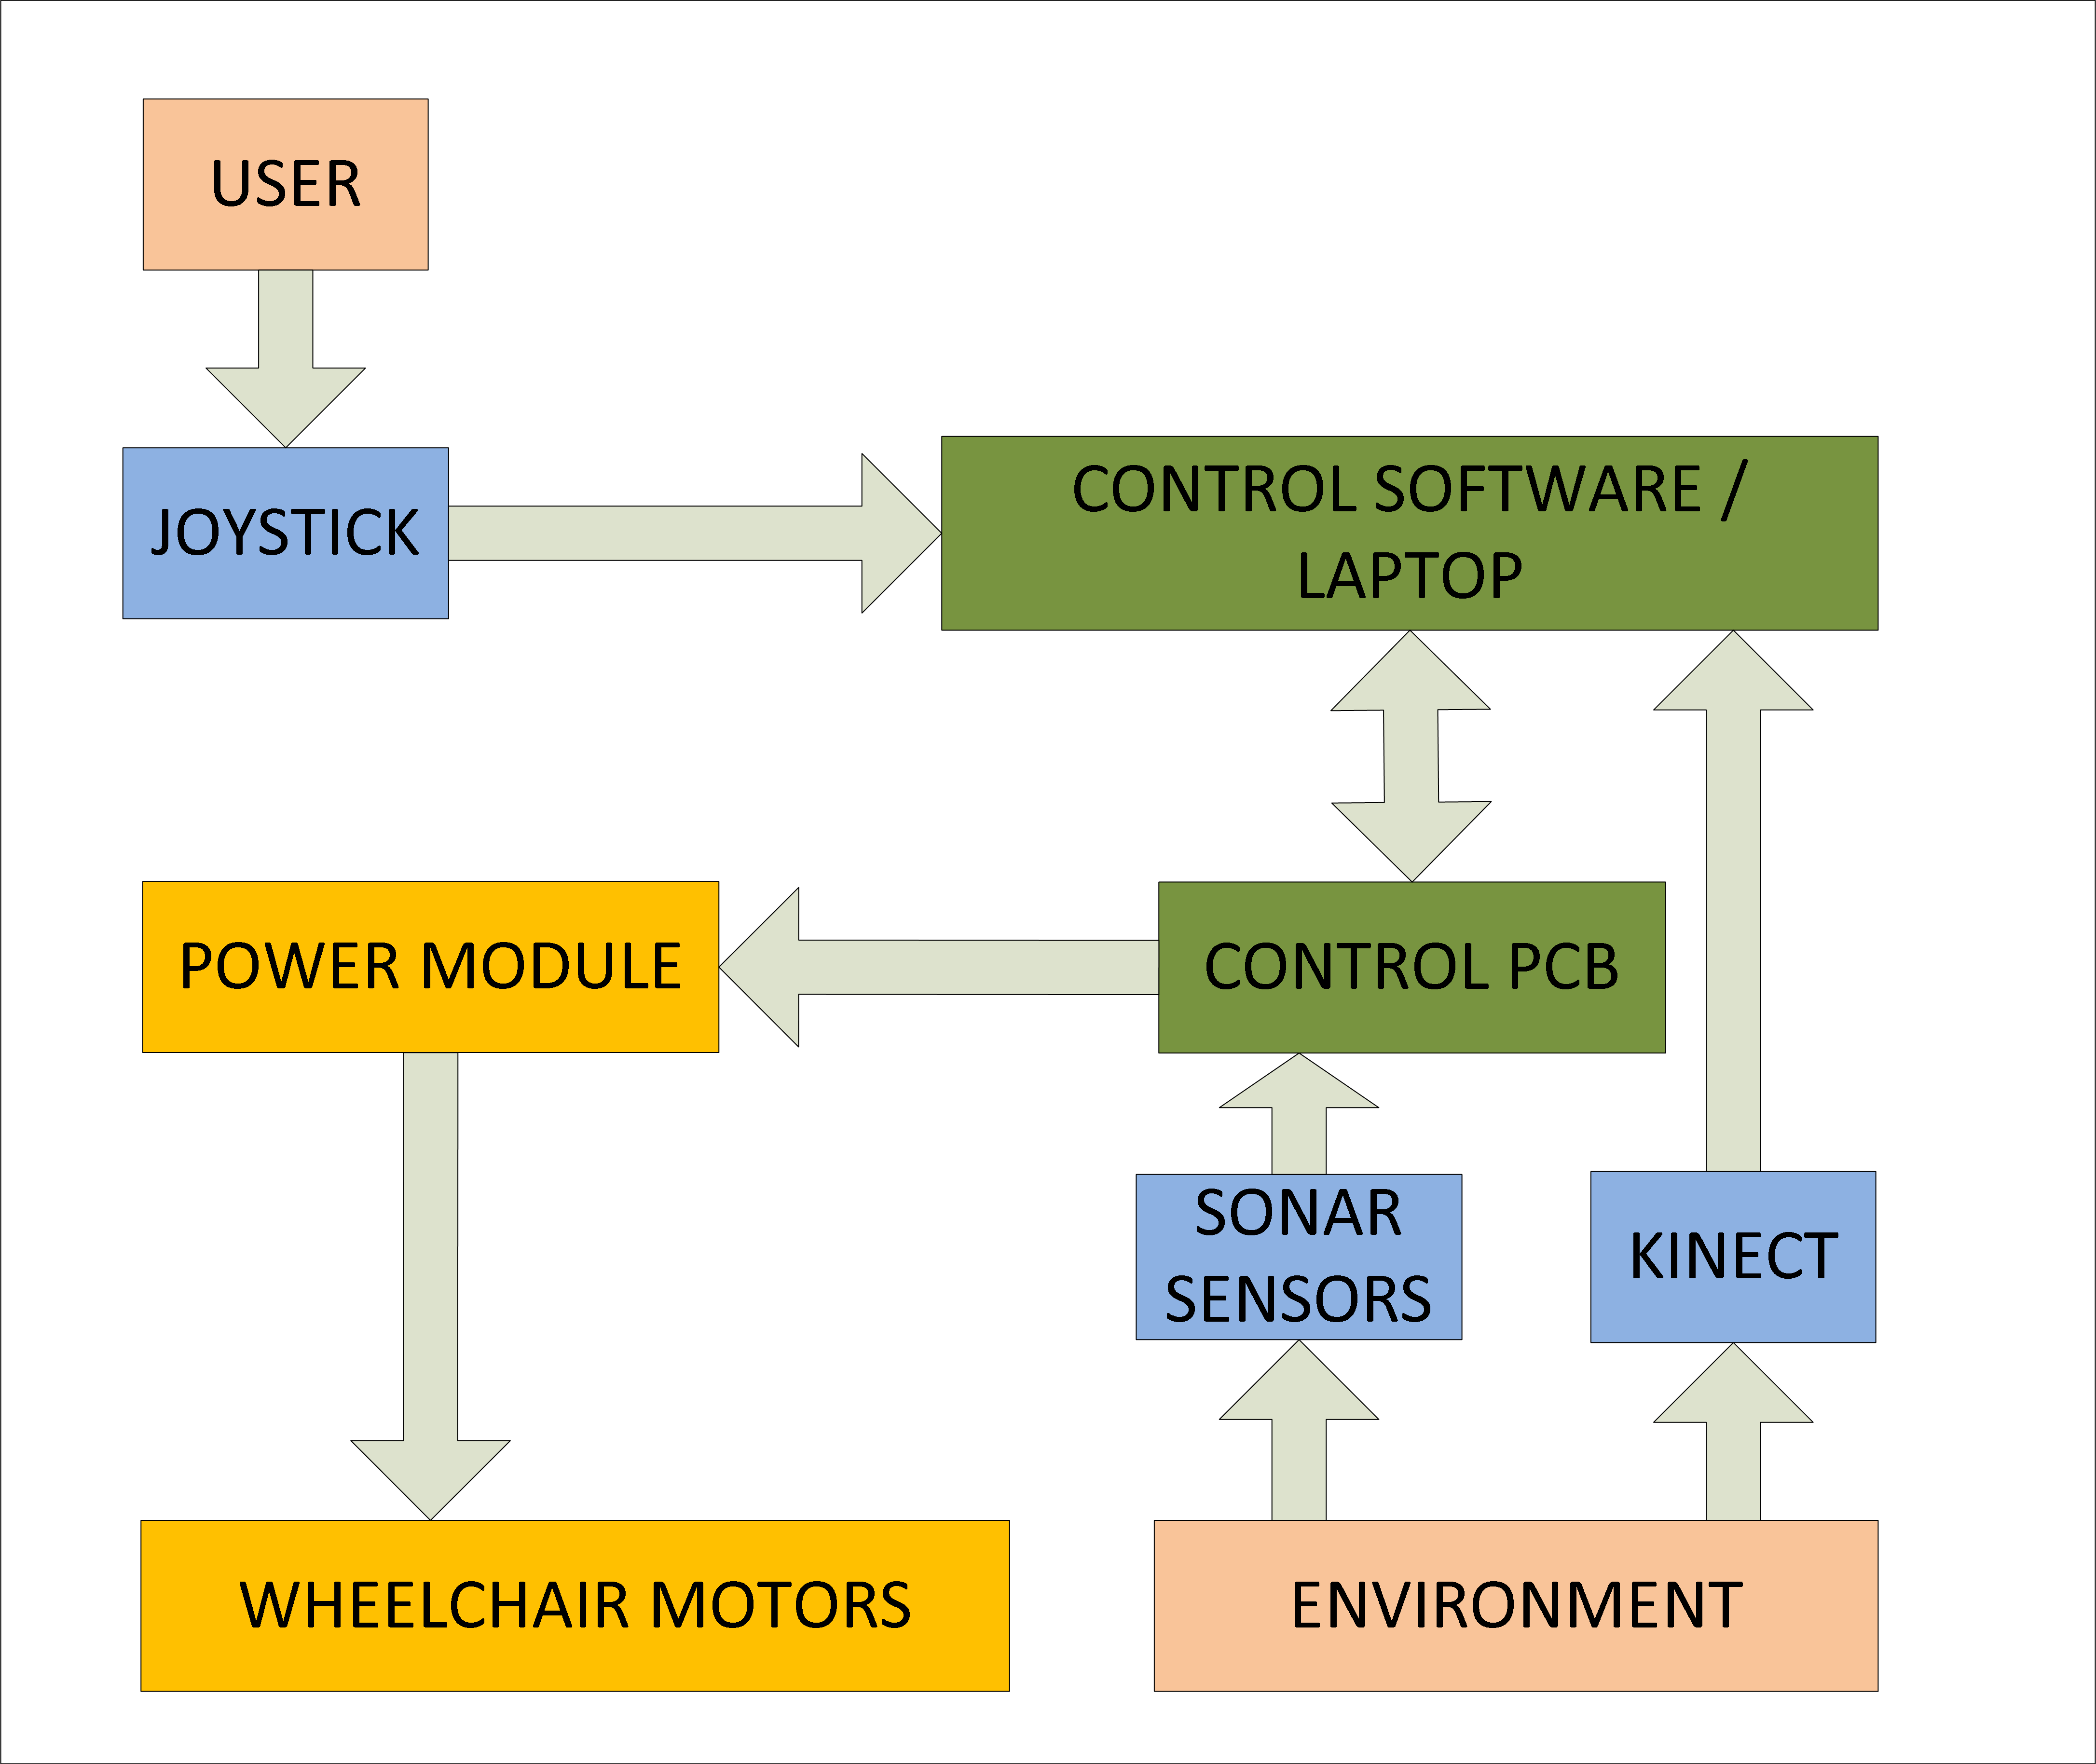
\includegraphics[scale=0.5]{System_Level}
 \caption{System Level Design}\label{fig:highlevel}
\end{figure}

%TODO(?)

\section{Mechanical Design}
%TODO(rowan)

\section{Sensor Configuration}
\begin{figure}[hbt]
 \centering
 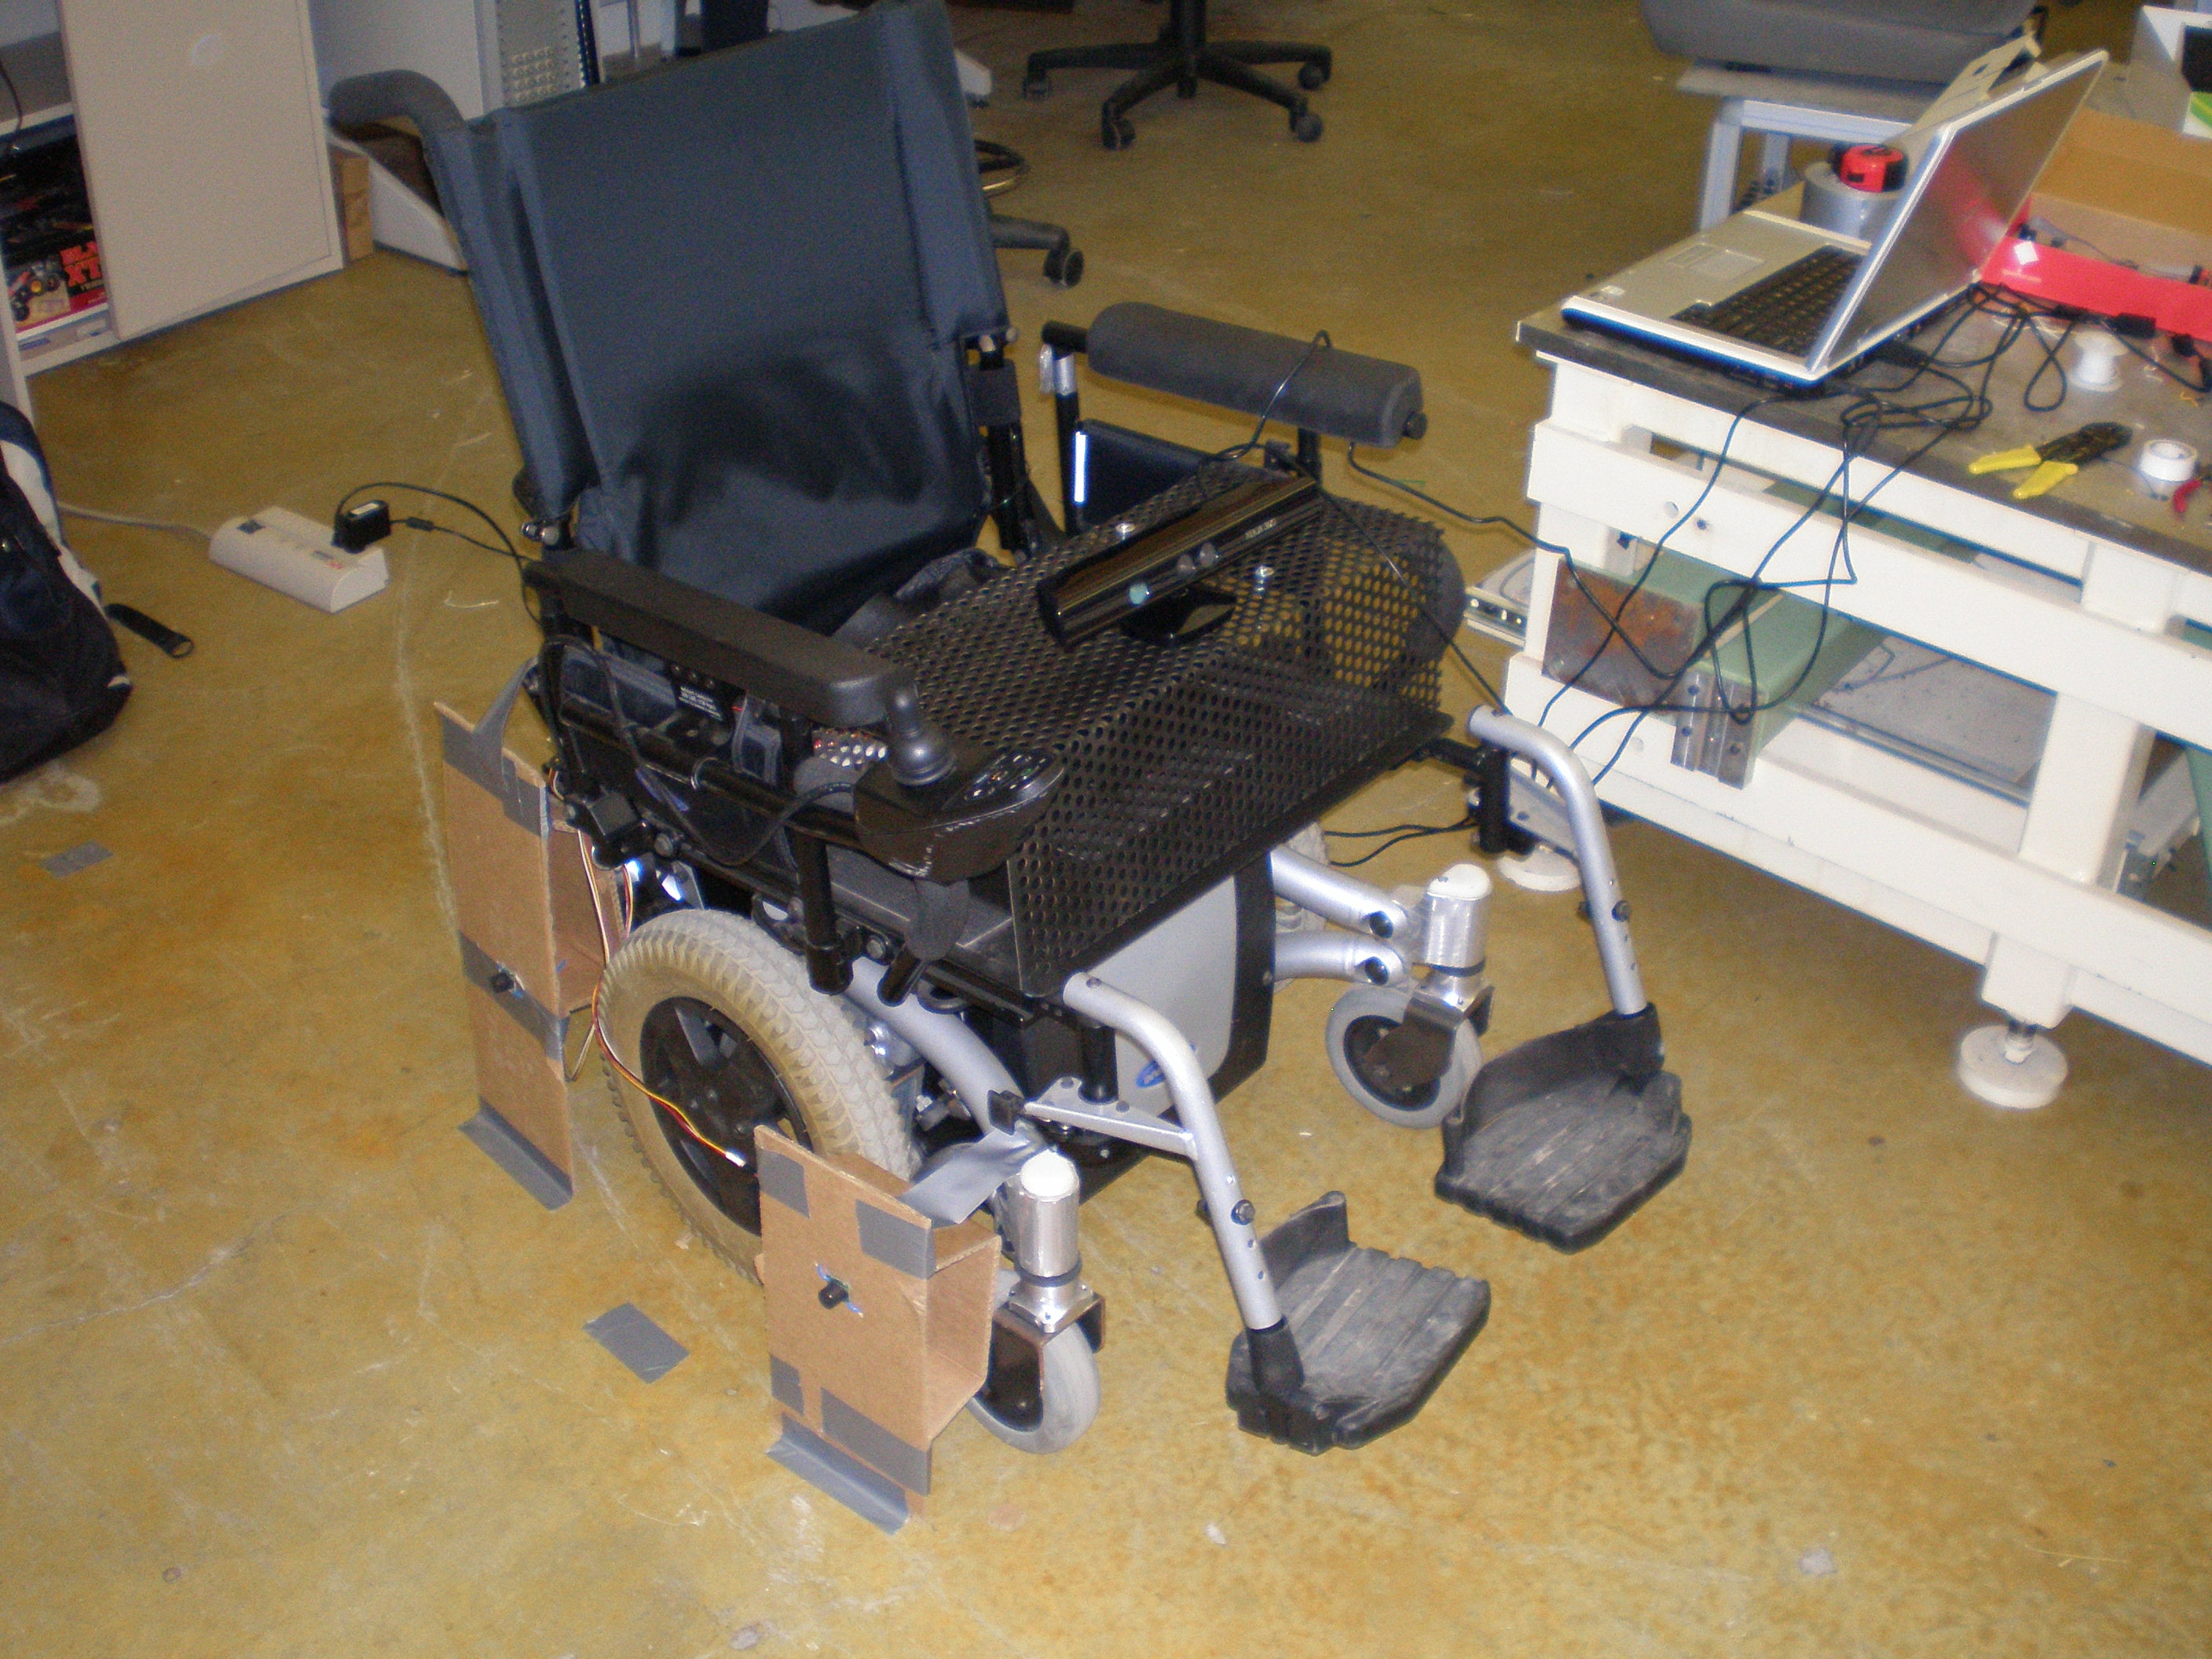
\includegraphics[scale=0.1]{testing}
 \caption{The sensor test set-up.}\label{fig:testing}
\end{figure}

\subsection{Kinect Configuration}
The Kinect sensor, based on the Primesense PS1080 System on Chip \cite{primesense}, provides a new type of depth sensing sensor. Previously projects requiring depth sensing measurements of both range and bearing (unlike ultrasonic or infrared rangers which give only range information) could use a laser rangefinder (LIDAR) or stereo-vision cameras. Laser rangefinders are both highly accurate and precise, but this comes at a very high monetary cost -- not reasonable for use in wheelchair collision avoidance technology that will be marketed to individuals and not research labs. Stereo-vision cameras require complex algorithms and lots of processing power to correspond features in images in order to identify disparities and get depth information out of this. This works out to a certain practical range -- limited by the spacing of the cameras being used and their resolution -- and is only good in areas with good lighting conditions and lots of unique features to correspond. Since the sensor is fairly new it makes sense to understand how it works, and what its accuracy and precision is, before determining the best final configuration.

The Primsense depth-sensor solution is shown in Figure \ref{fig:primesense_solution}. The Kinect presents something of a combination between the lidar and the stereo vision depth mapping techniques, sending out coded infrared light (similar to a lidar) and reading back the response on a standard CMOS image sensor (which keeps things very cheap). The solution does all its processing on board the PS1080, and sends the fully-processed depth map information back to the host. The result is reasonable accuracy and precision (for this application), and low price. Note that while the Xbox Kinect from Microsoft is being used for the prototype of this collision aviodance project, there are other manufacturers of depth sensors using the Primesense technology on the market that could eventually be used to reduce cost for production purposes.

\begin{figure}[hbt]
 \centering
 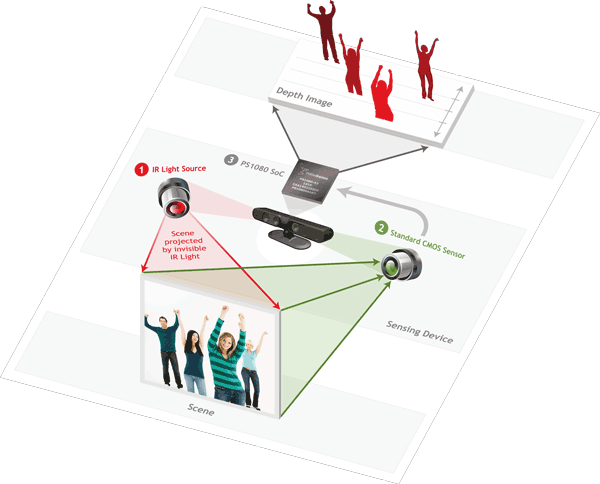
\includegraphics[scale=0.35]{PrimeSensor_Depth_Diagram}
 \caption{The Primesense system \cite{primesense}} \label{fig:primesense_solution}
\end{figure}

The Kinect comes with a set of camera calibration parameters, and the software available from OpenNI \cite{OpenNI} and the Robot Operating System (ROS) \cite{ROS} package that supports the Kinect have gone to great lengths to provide a good calibration for the depth camera. The result is that the accuracy of the sensor is within  $\pm 1$ 1 cm of the true measurement, and with custom calibration with $\pm 1$ mm over its range of operation \cite{kinect_prec}.

The precision is less good (though still not bad at all) and increases with the square of distance. This is shown in Figure \ref{fig:kinect_precision} provided by \cite{kinect_prec}. However, for the application of collision avoidance very high precision data is not required, and we can see that even out to 2 meters of range the 95th percentile of data falls with 2.5 cm of the true range. It will quickly fall off in precision with range, but the wheelchair does not need to react very quickly to data that is farther away, and in tight spots the wheelchair will be close to obstacles and hence get very precise data from sensor.

\begin{figure}[hbt]
 \centering
 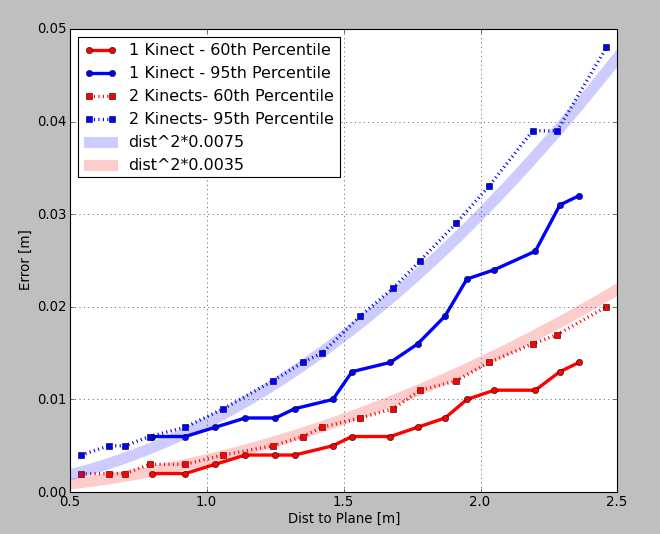
\includegraphics[scale=0.35]{kinect_precision}
 \caption{Kinect Sensor Precision \cite{kinect_prec}} \label{fig:kinect_precision}
\end{figure}

To prove out the operation of the Kinect sensor, the test setup shown in Figure \ref{fig:testing}. The authors stood in front of the camera at a few meters of range and a set of data was gathered. This data is shown in the format of a point cloud \cite{point_clouds} in Figure \ref{fig:groupPCL}. A point cloud is a set of (X,Y,Z) coordinates that represents the depth (Z) of a point at each (X,Y) coordinate on the map. This is provided to us in meters, being converted from the camera perspective to the world (X,Y,Z) frame transparently by using ROS and the OpenNI Kinect node that comes as  "node", a program that operates in the ROS environment.

\begin{figure}[hbt]
 \centering
 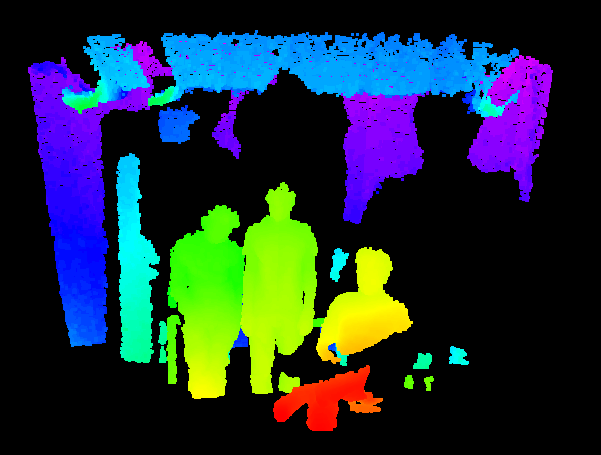
\includegraphics[scale=0.35]{group_pointcloud}
 \caption{Kinect Point Cloud Sample} \label{fig:groupPCL}
\end{figure}

The problem with this point cloud data is that it can include floor and ceiling measurements (as seen in Figure \ref{fig:groupPCL} that are clearly not obstacles. Also, if the camera is not pointing parallel to the floor the "world" coordinate frame axes used to construct the point cloud will not be lined up with ground plane (a level floor in the case of a wheelchair).

The solution is to first transform the point cloud data into the true world coodinate frame using a simple rotation matrix. The desired rotation can either be read from the accelerometer in the Kinect sensor (by measuring the gravity vector), finding a plane of best fit using an image of the floor, or just calibrating the sensor once at the time of manufacture when it is fixed to the wheelchair. Then only a slice of the point cloud is considered, the one above the floor plane but below what would be considered the top of the wheelchair. This slice is projected onto a course grid where any points within a box cause an object to be indicated, and otherwise the box is considered free space. The occupancy grid for Figure \ref{fig:groupPCL} is shown in Figure \ref{fig:groupOccupancy}.

\begin{figure}[hbt]
 \centering
 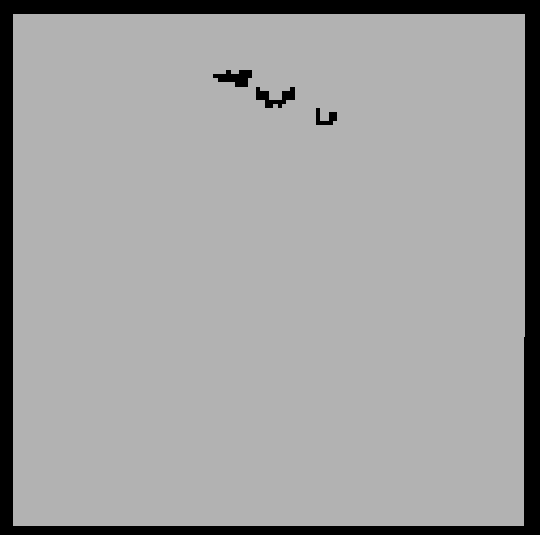
\includegraphics[scale=0.35]{group_occupancy}
 \caption{Kinect Occupancy Grid Sample} \label{fig:groupOccupancy}
\end{figure}

The occupancy grid shows free space (grey) and obstacles (black). Comparing Figure \ref{fig:groupPCL} to Figure \ref{fig:groupOccupancy} we can see the torsos of two individuals and the head of a third shown in the occupancy map. This is because the slice closen to be projected onto the grid was a 30 cm range about the center of the image, at approximately the head height of the seated individual. In practice, this range with be tuned to avoid accidental measurments from the floor and extend up to the height of the wheelchair to reject false obstacles such as the floors and ceilings.

This proves the concept works well, and only some tuning of the constants will be required to integrate the Kinect with the final prototype.

\section{Rangefinder Configuration}
SONAR sensors which were available on-hand were used to test a number of configurations.  The sensors used were the MaxBotix LV-EZ4.  These sensors are designed to be sensitive to object only within a cylindrical region of about 60 cm diameter \cite{lv-ez4}.  

Figures \ref{sonar_1} - \ref{sonar_3} show the results of testing with the LV-EZ4.  Unsurprisingly, area coverage is poor with the narrow-beam sensor.  The best results are observed in figure \ref{sonar_2}, where the forward field is fully covered.

\begin{figure}[hbt]
 \centering
 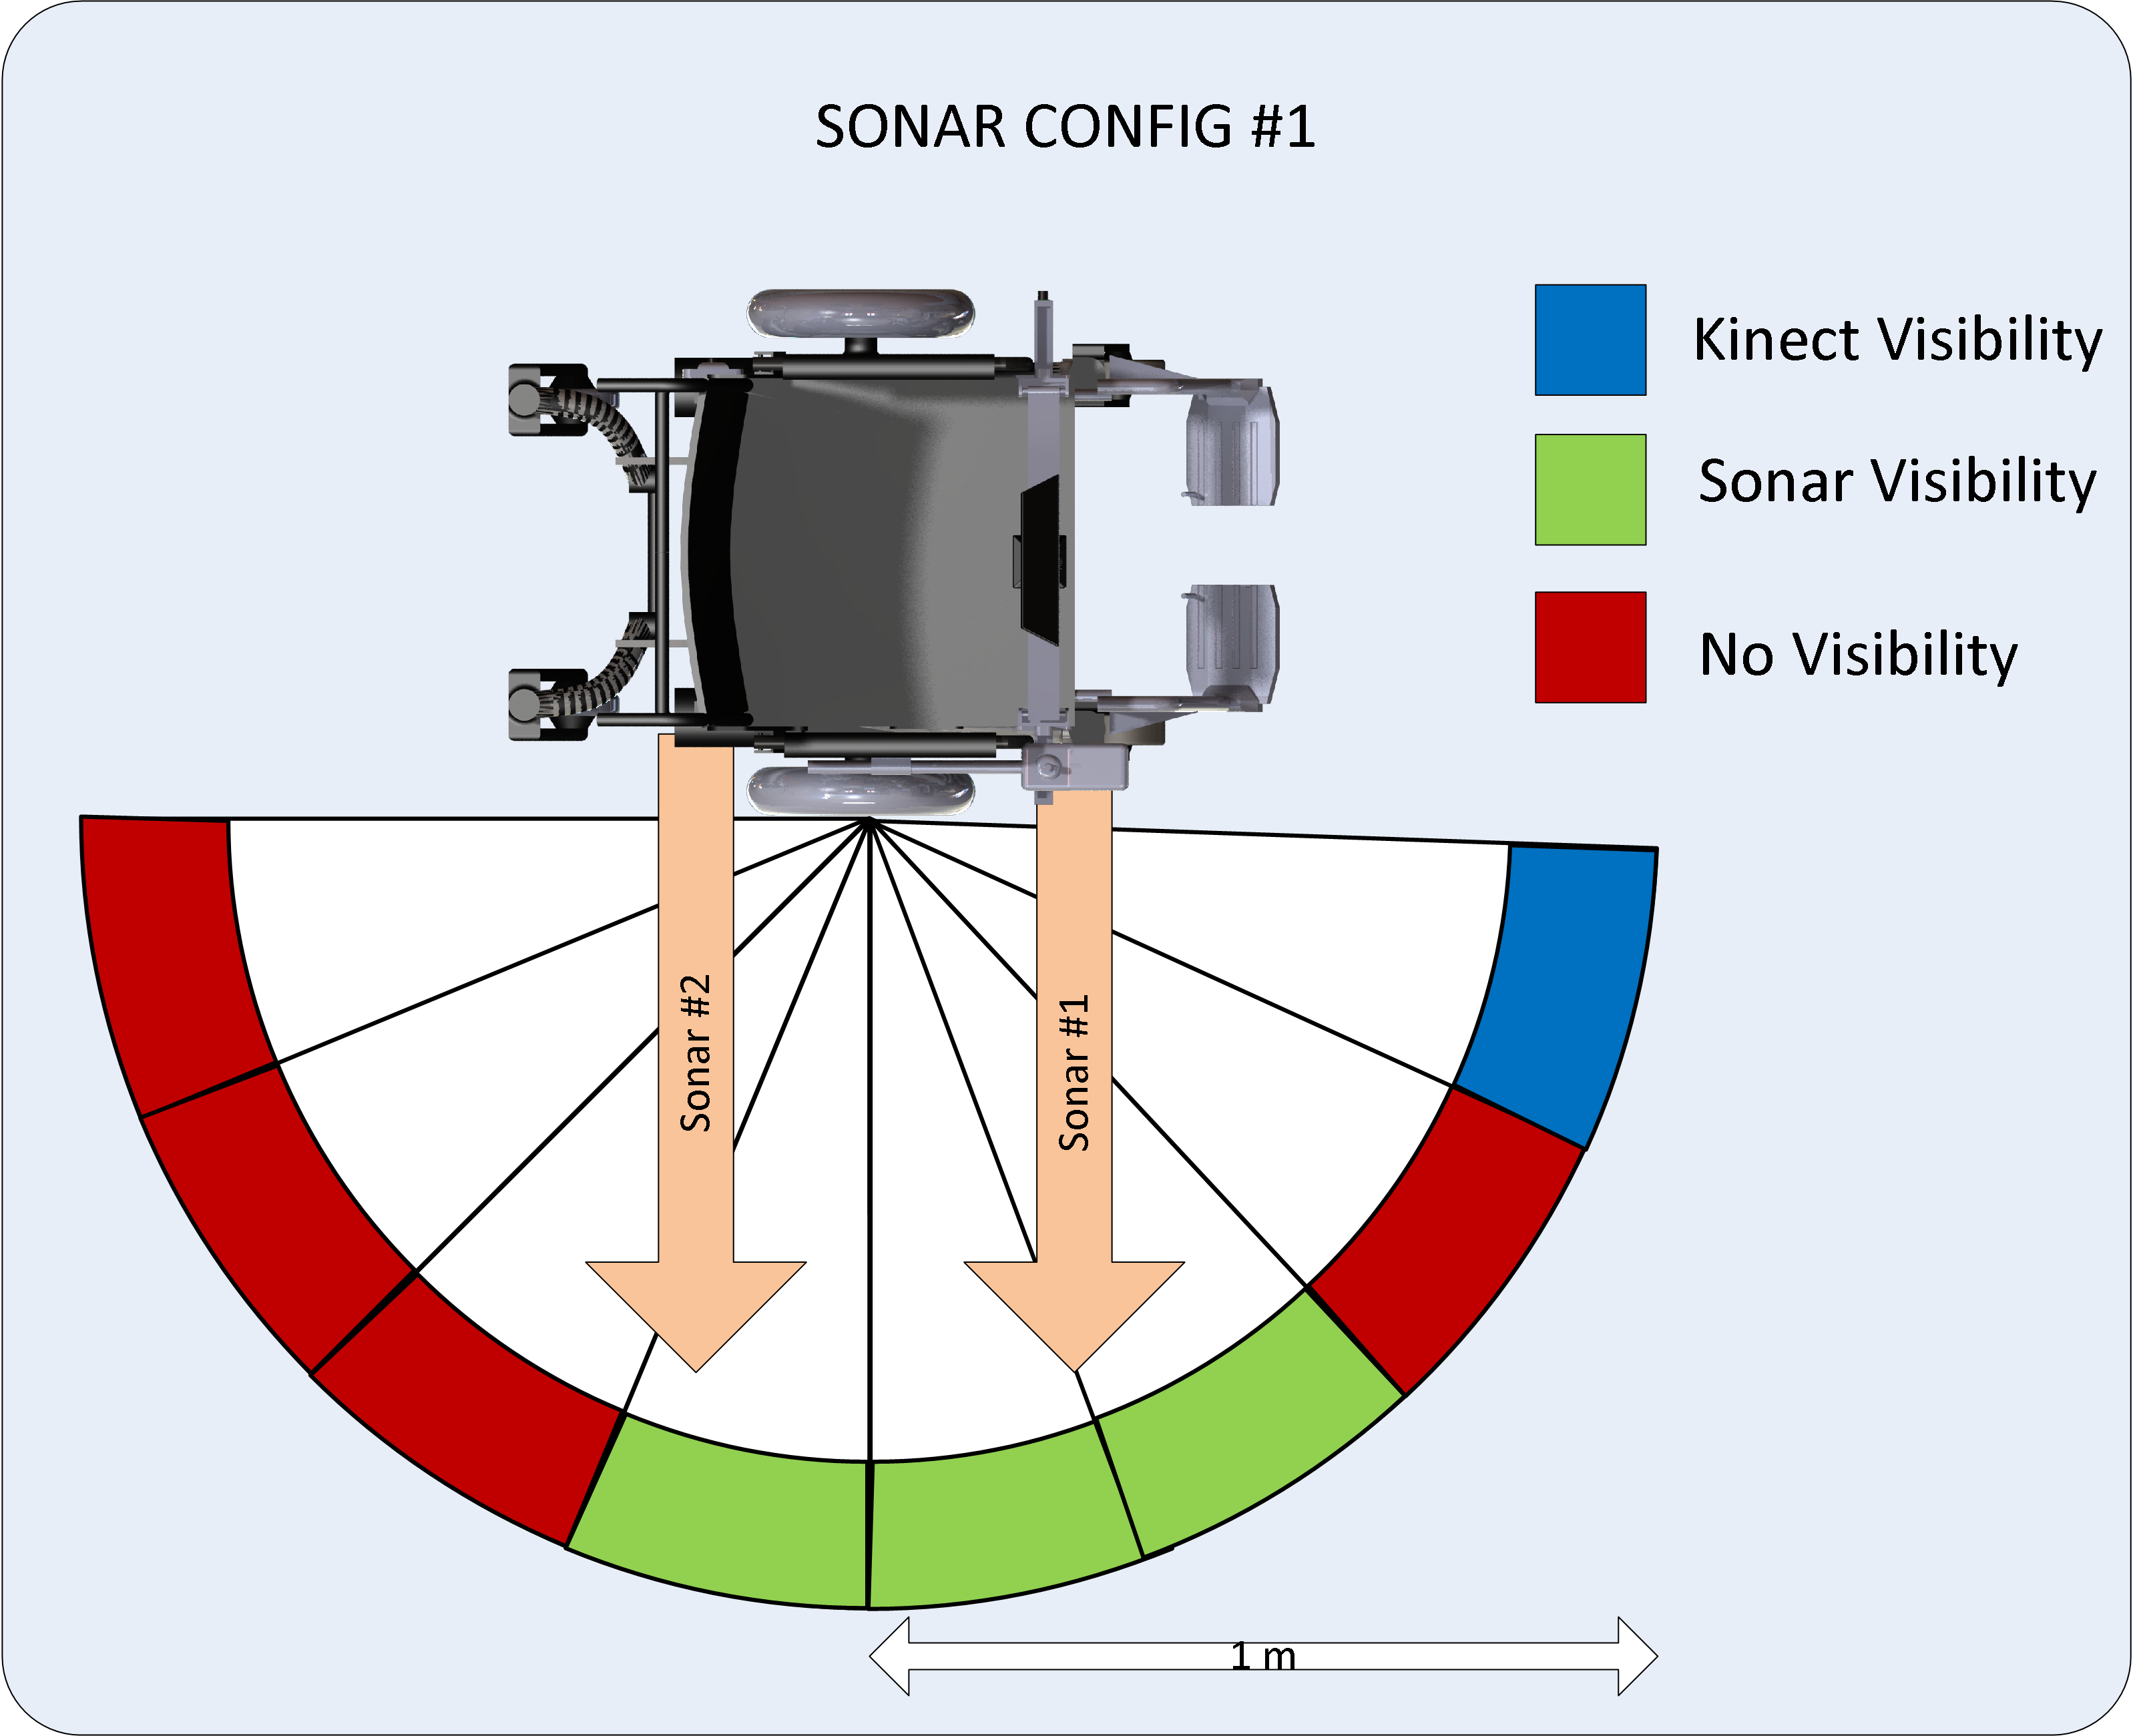
\includegraphics[scale=0.6]{SONAR_Config1.png}
 \caption{SONAR test configuration 1.}
 \label{sonar_1}
\end{figure}

\begin{figure}[hbt]
 \centering
 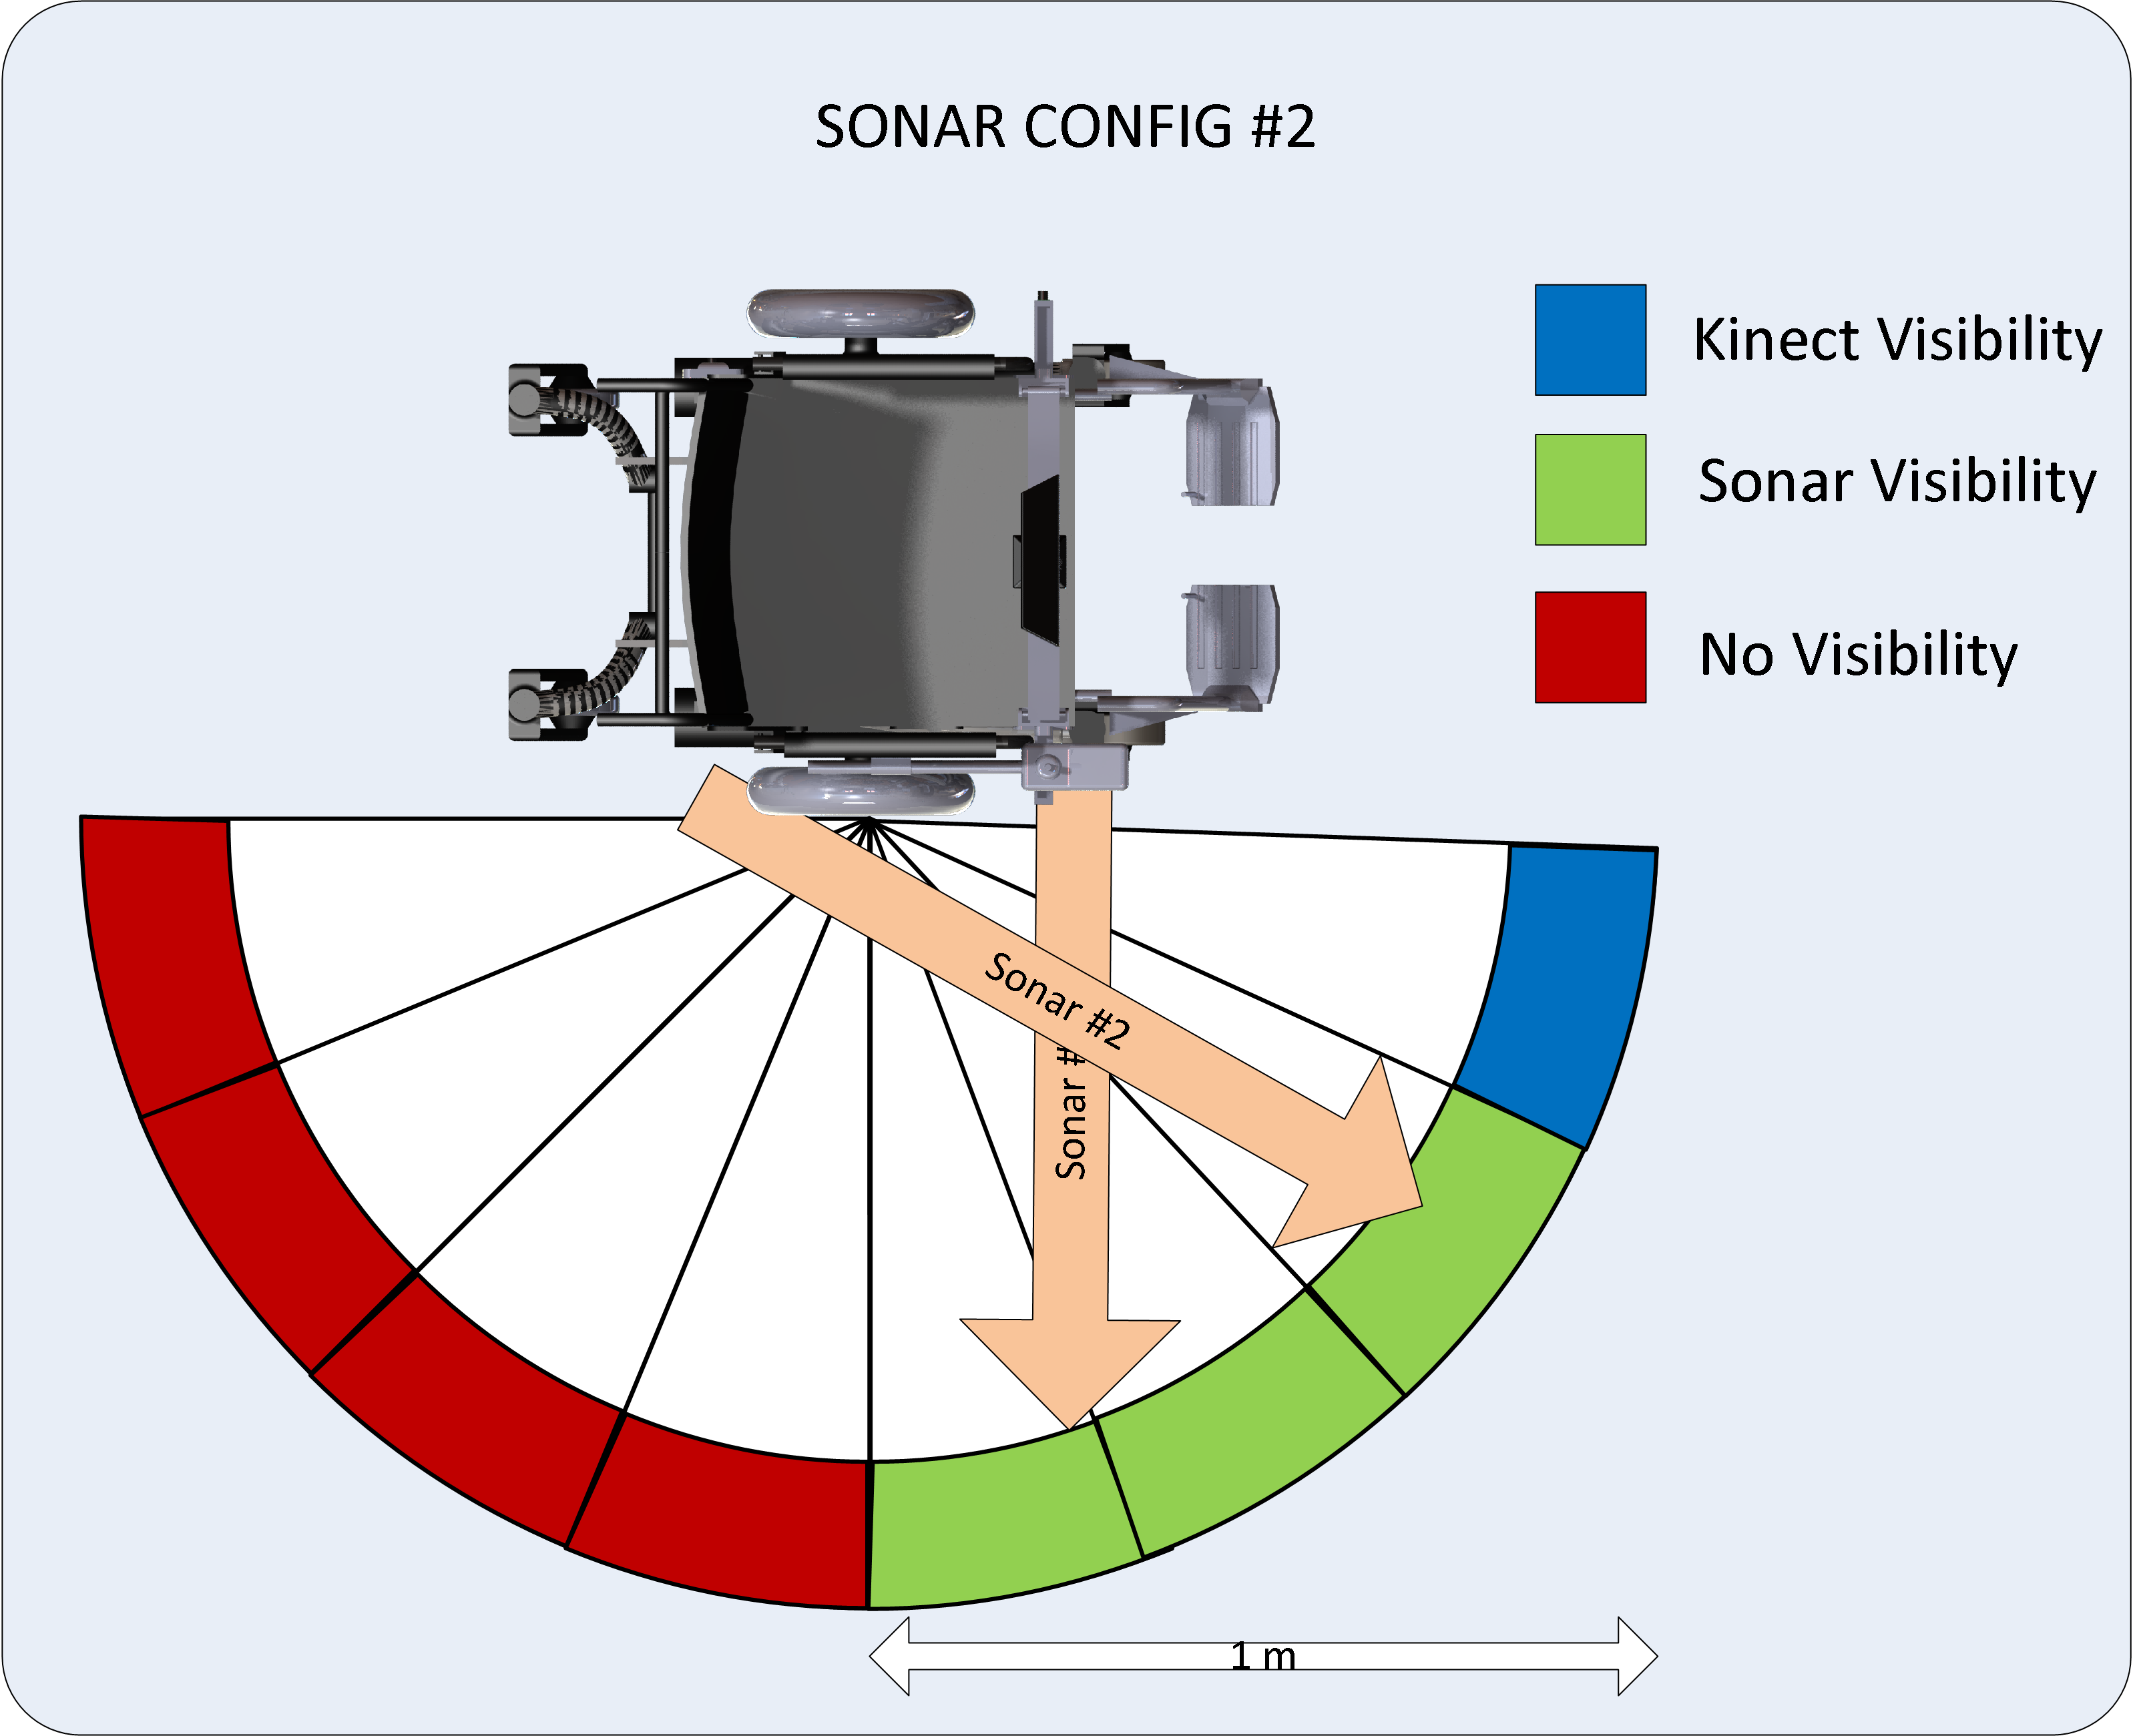
\includegraphics[scale=0.6]{SONAR_Config2.png}
 \caption{SONAR test configuration 2.}
 \label{sonar_2}
\end{figure}

\begin{figure}[hbt]
 \centering
 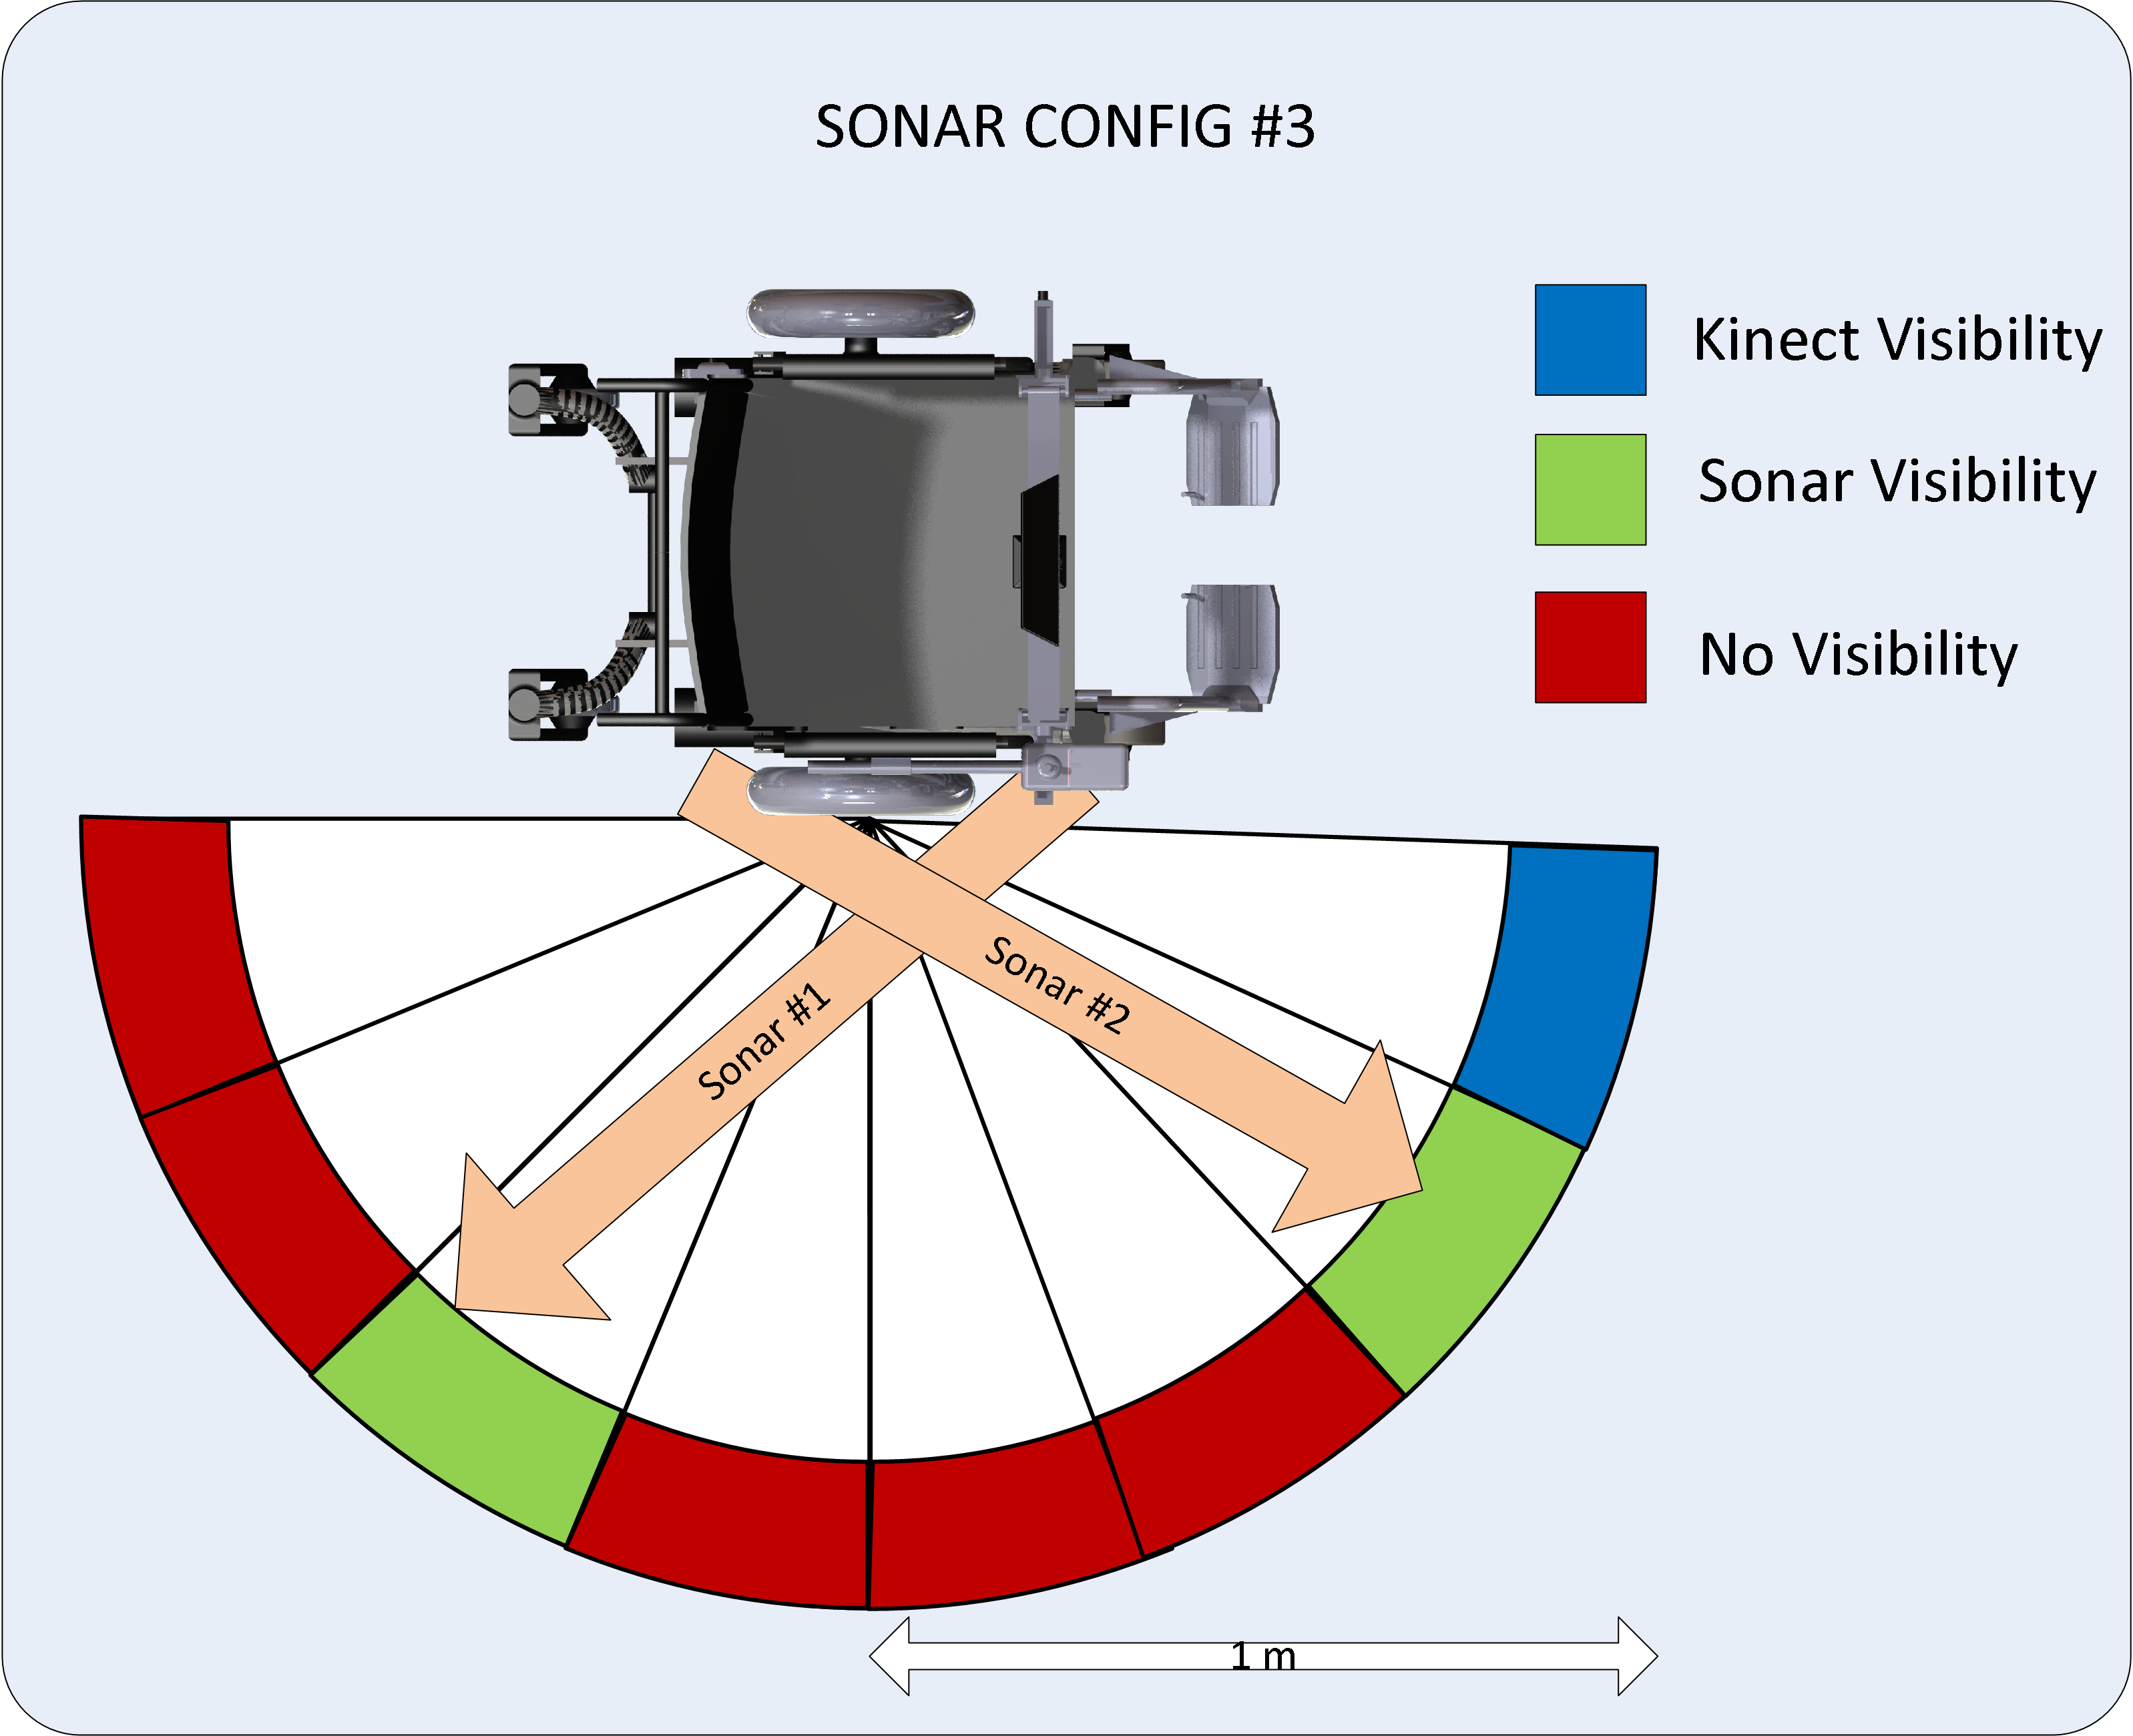
\includegraphics[scale=0.6]{SONAR_Config3.png}
 \caption{SONAR test configuration 3.}
 \label{sonar_3}
\end{figure}

Considering the poor coverage provided by the narrow-beam LV-EZ4 sensors, it is recommended that wider range sensors be used.  For cylindrical objects, the EZ0 model of the same series is sensitive within a cone of approximately $60^\circ$ \cite{lv-ez0}.  Note that, although region of sensitivity depends on object shape, observations indicate that humans are well approximated by large cylindrical dowels.  

With the LV-EZ0 sensors, it is expected that it will be possible to achieve good lateral visibility. Figure \ref{sonar_final} shows the coverage we expect with these sensors.

\begin{figure}[hbt]
 \centering
 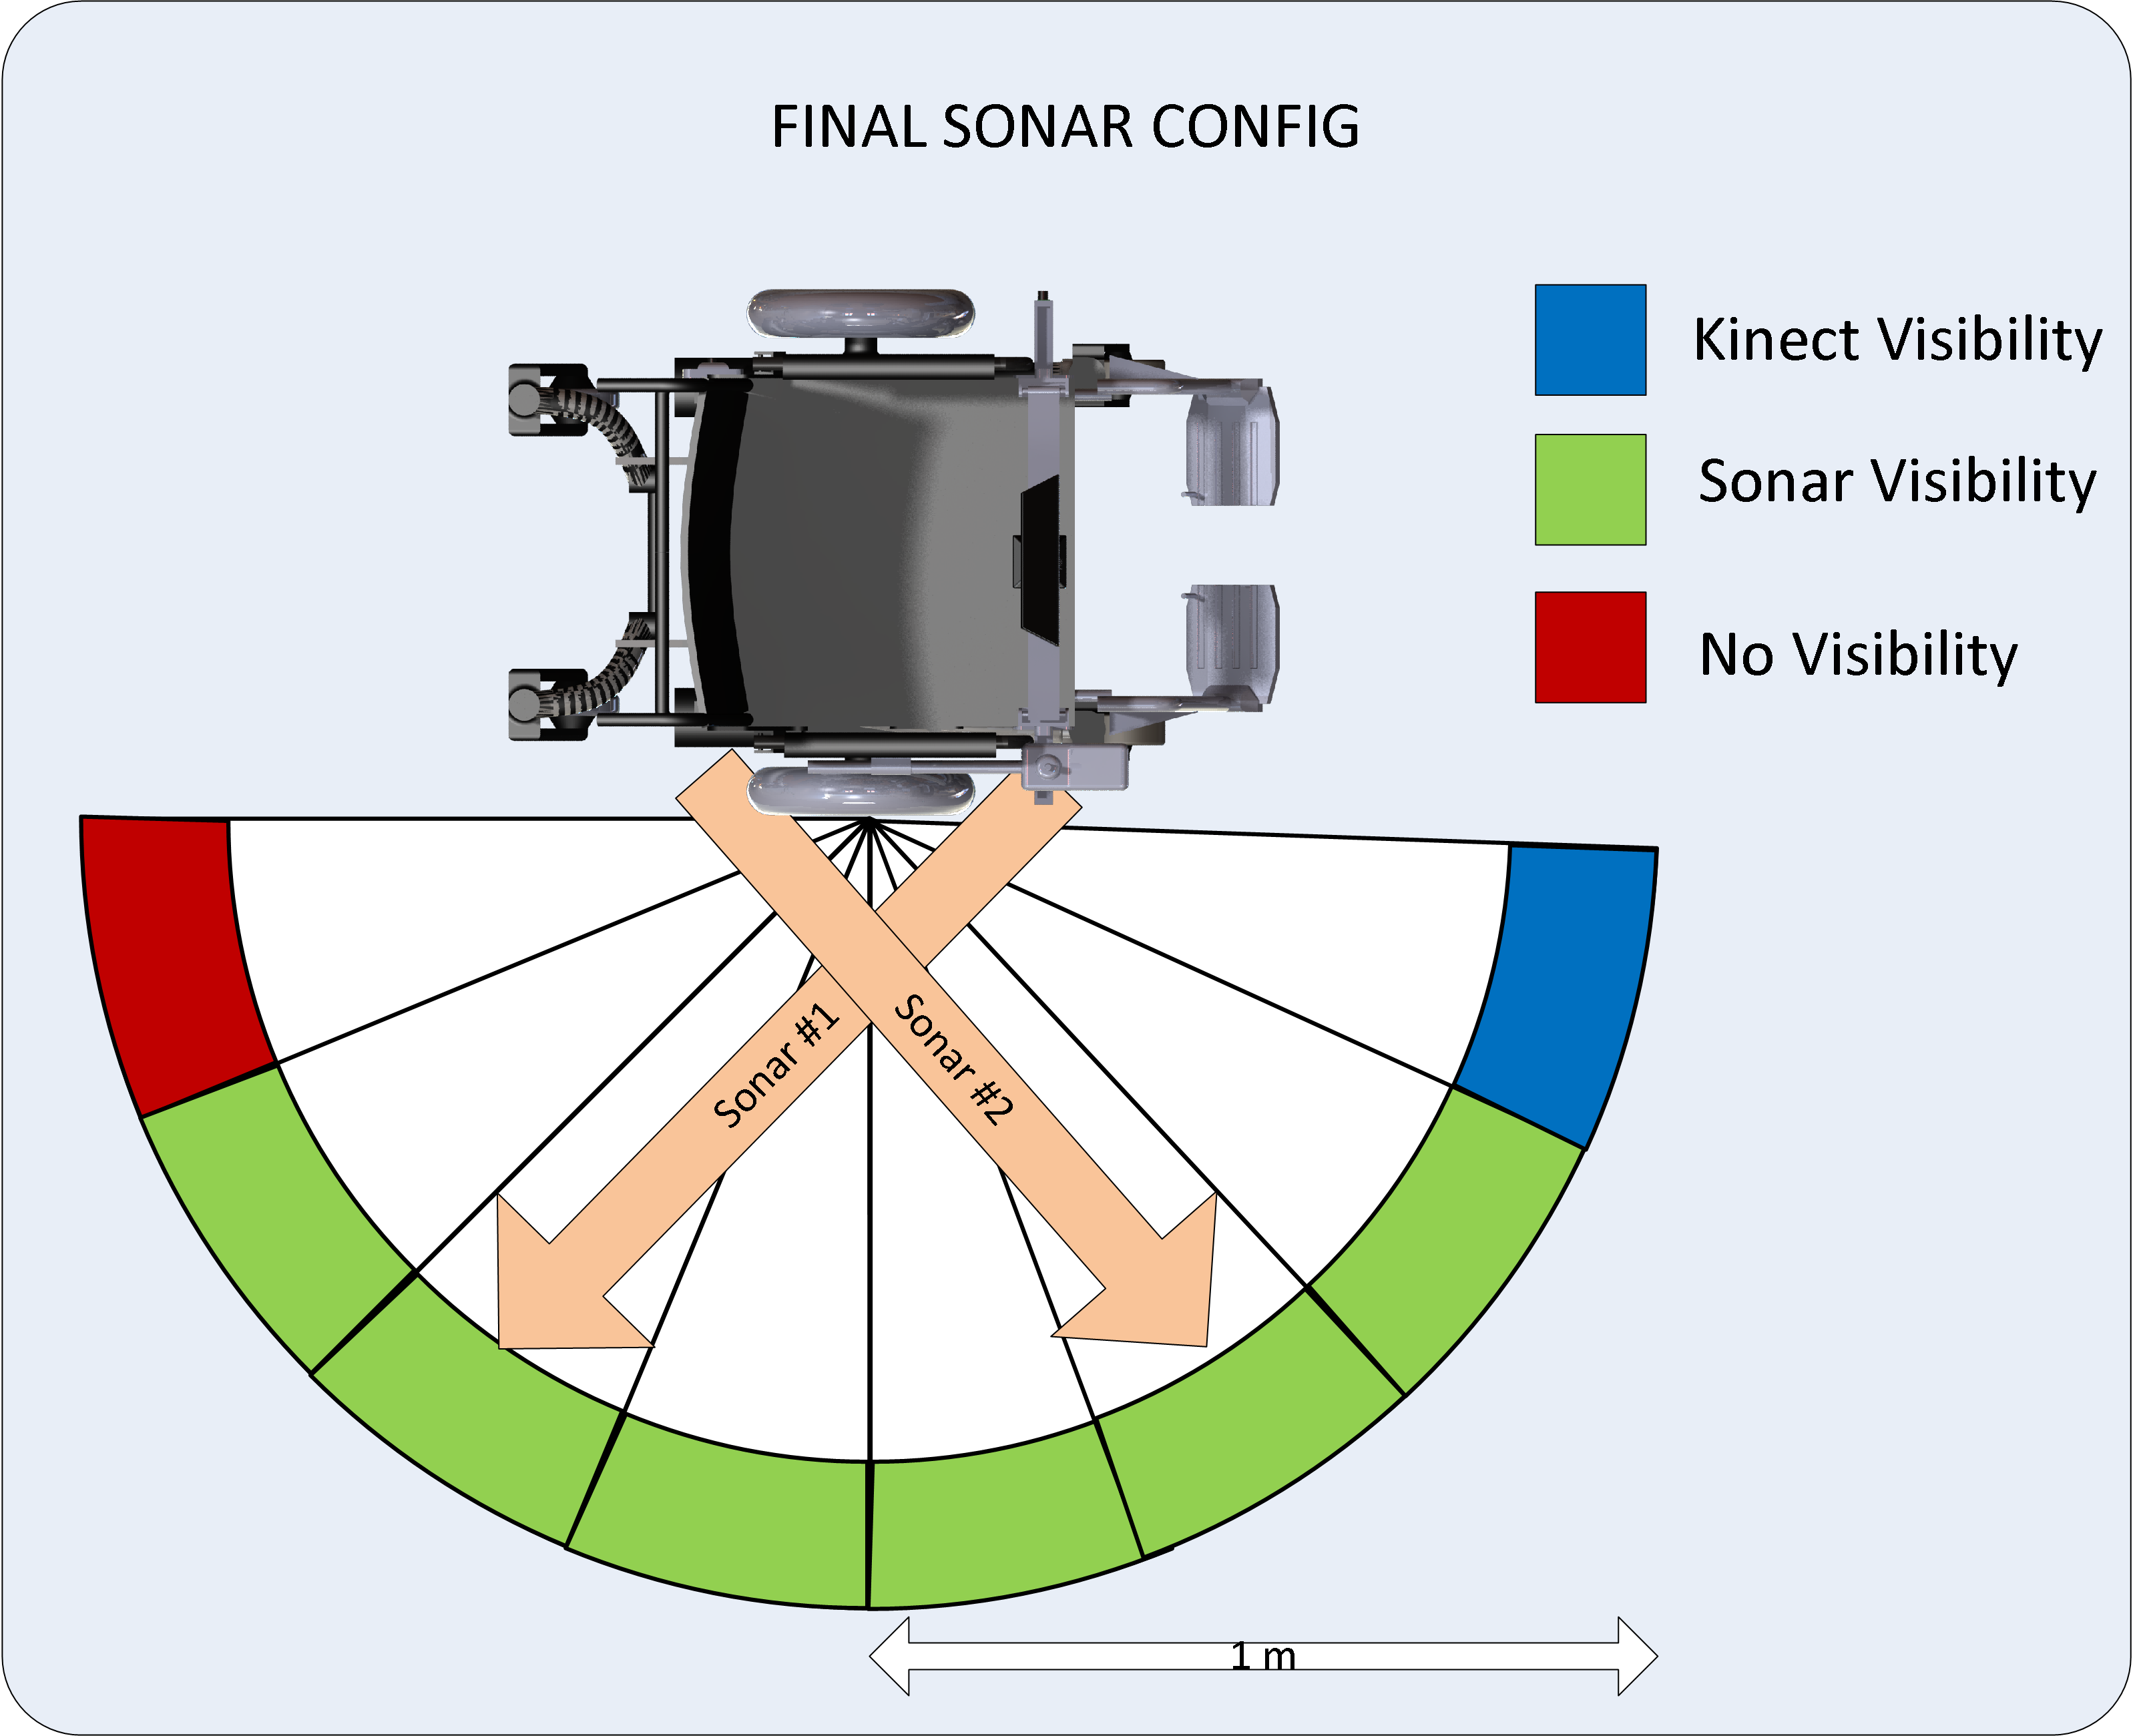
\includegraphics[scale=0.6]{SONAR_Config_Final.png}
 \caption{Final SONAR configuration.}
 \label{sonar_final}
\end{figure}


\section{Systems Integration}
%TODO(iain/jordan)

\section{Hardware Design}
\begin{figure}[hbt]
 \centering
 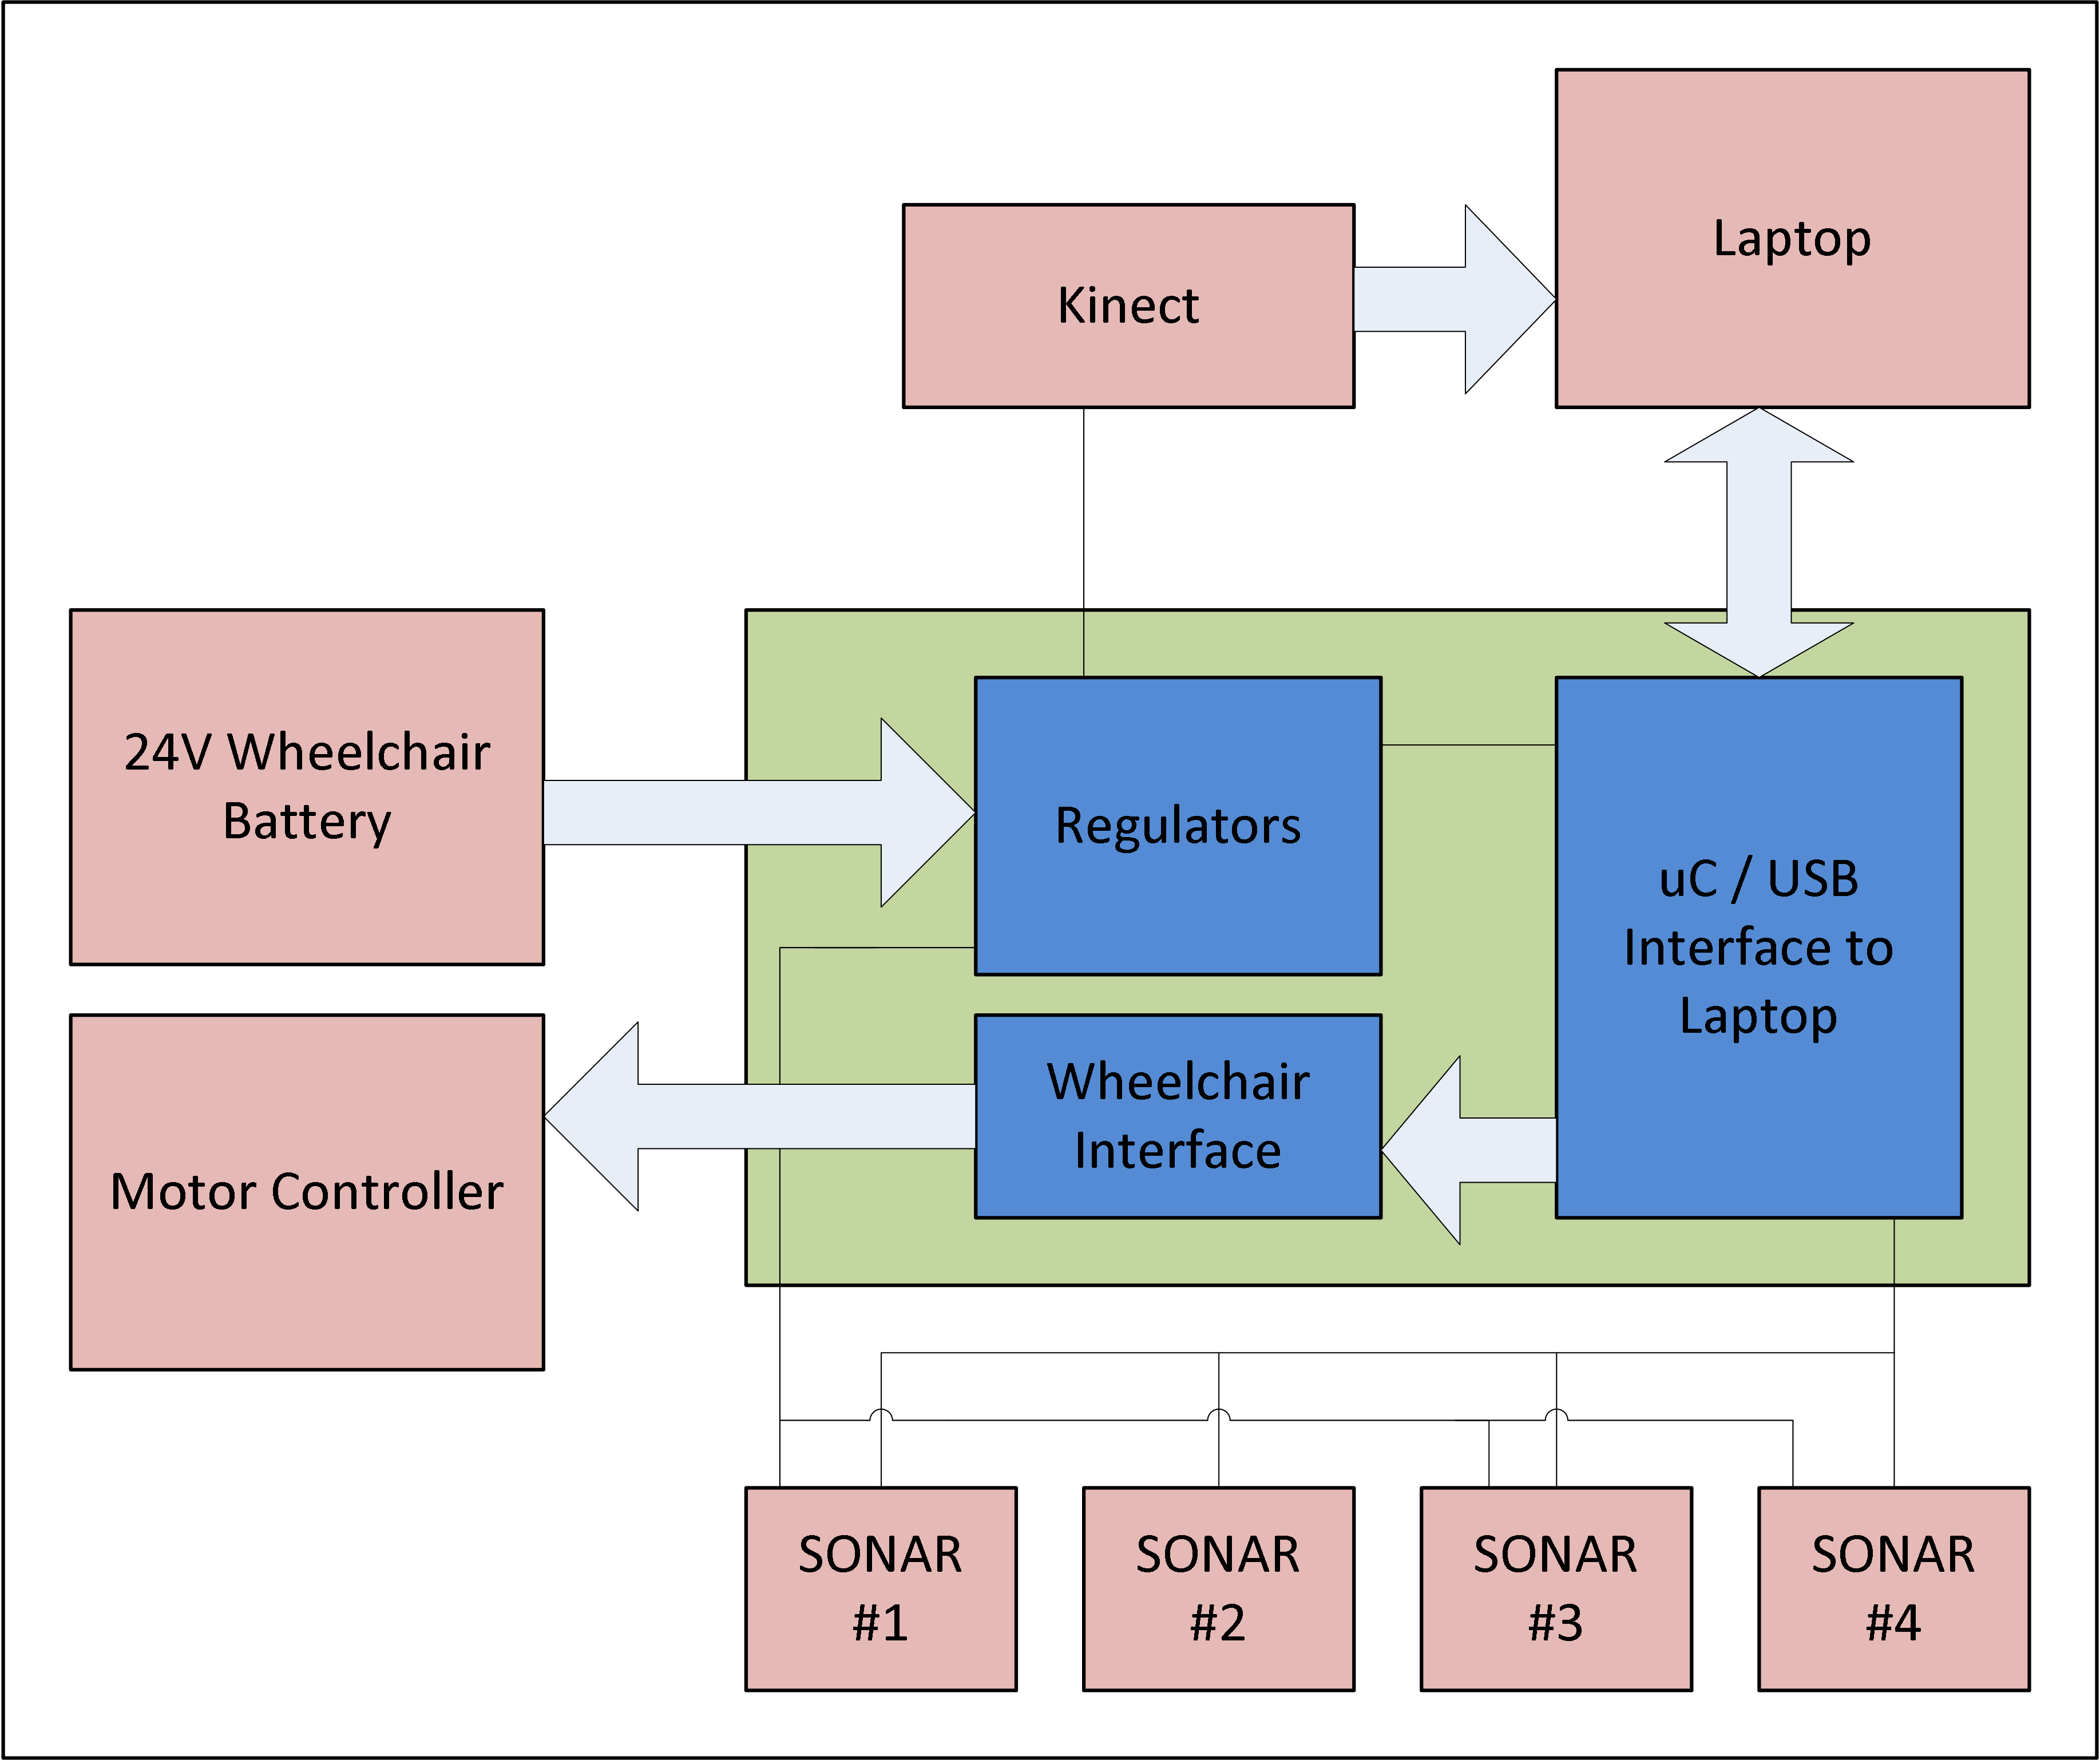
\includegraphics[scale=0.5]{Hardware_Diagram}
 \caption{Hardware Design}\label{fig:hardware}
\end{figure}

\section{Software Design}
\begin{figure}[hbt]
 \centering
 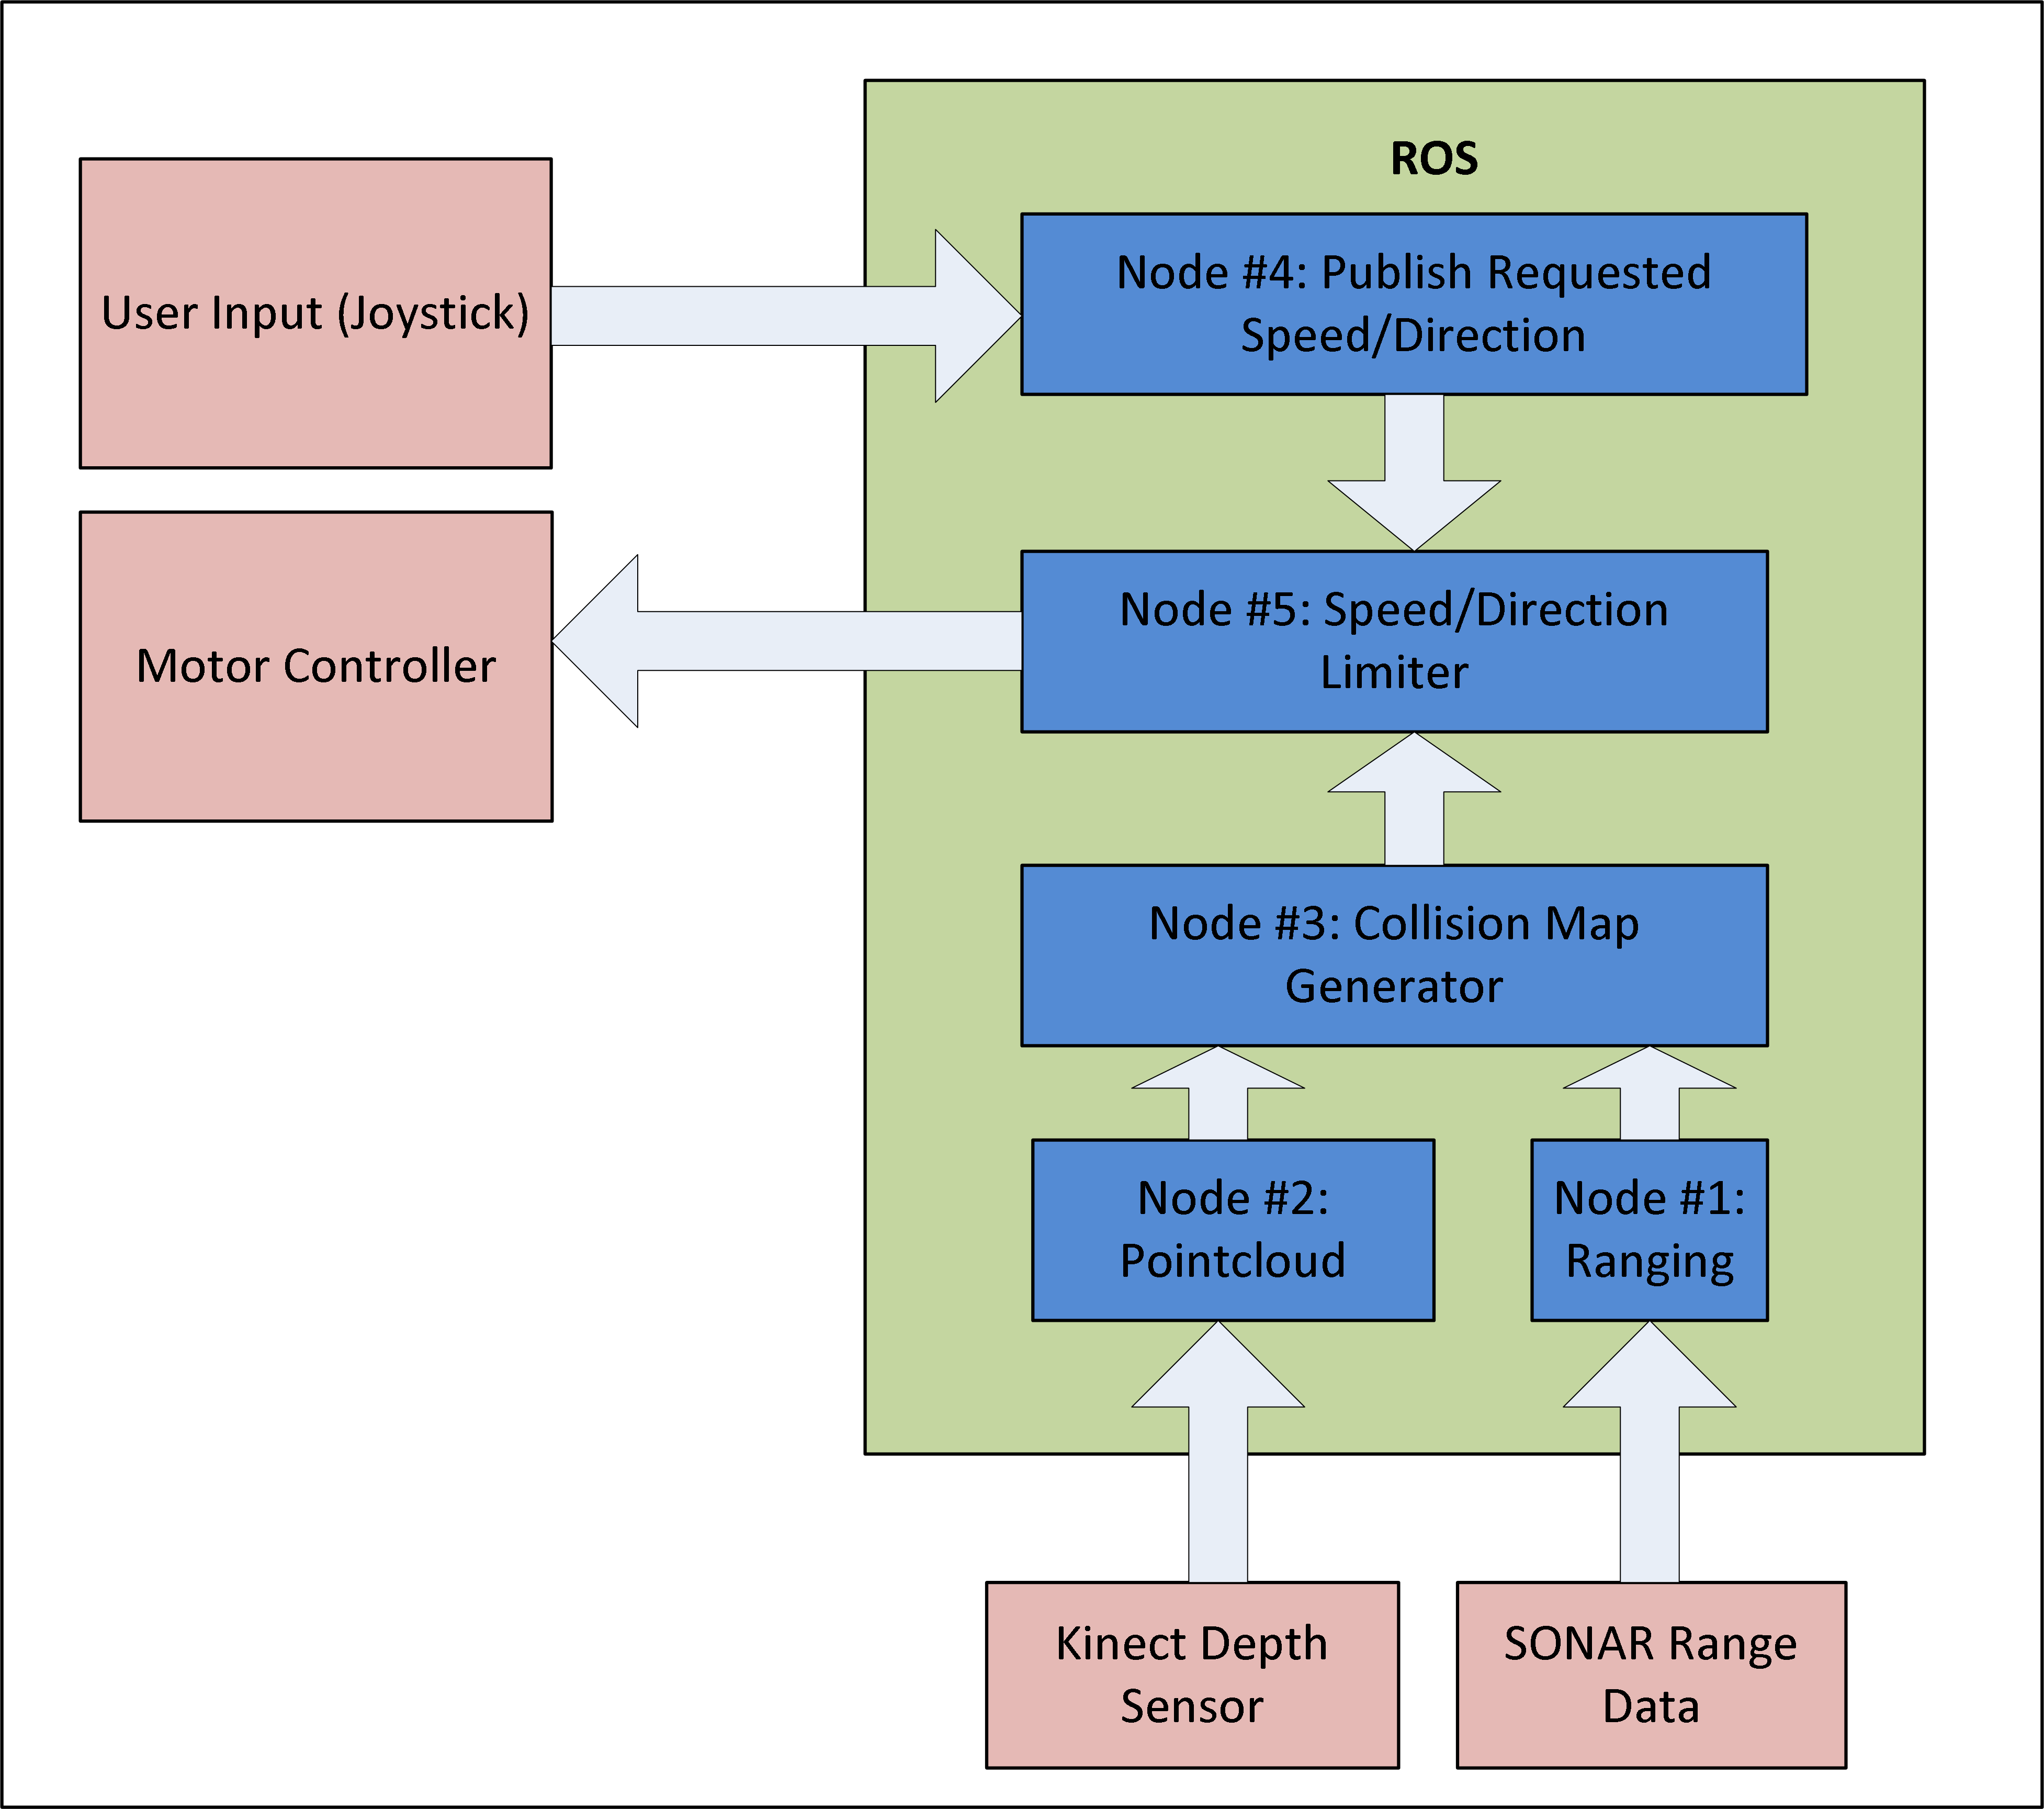
\includegraphics[scale=0.5]{Software_Diagram}
 \caption{Software Design}\label{fig:software}
\end{figure}
%TODO(iain/jordan)

\chapter{Schedule and Budget}

\section{Schedule}
\begin{figure}[htb]
 \centering
 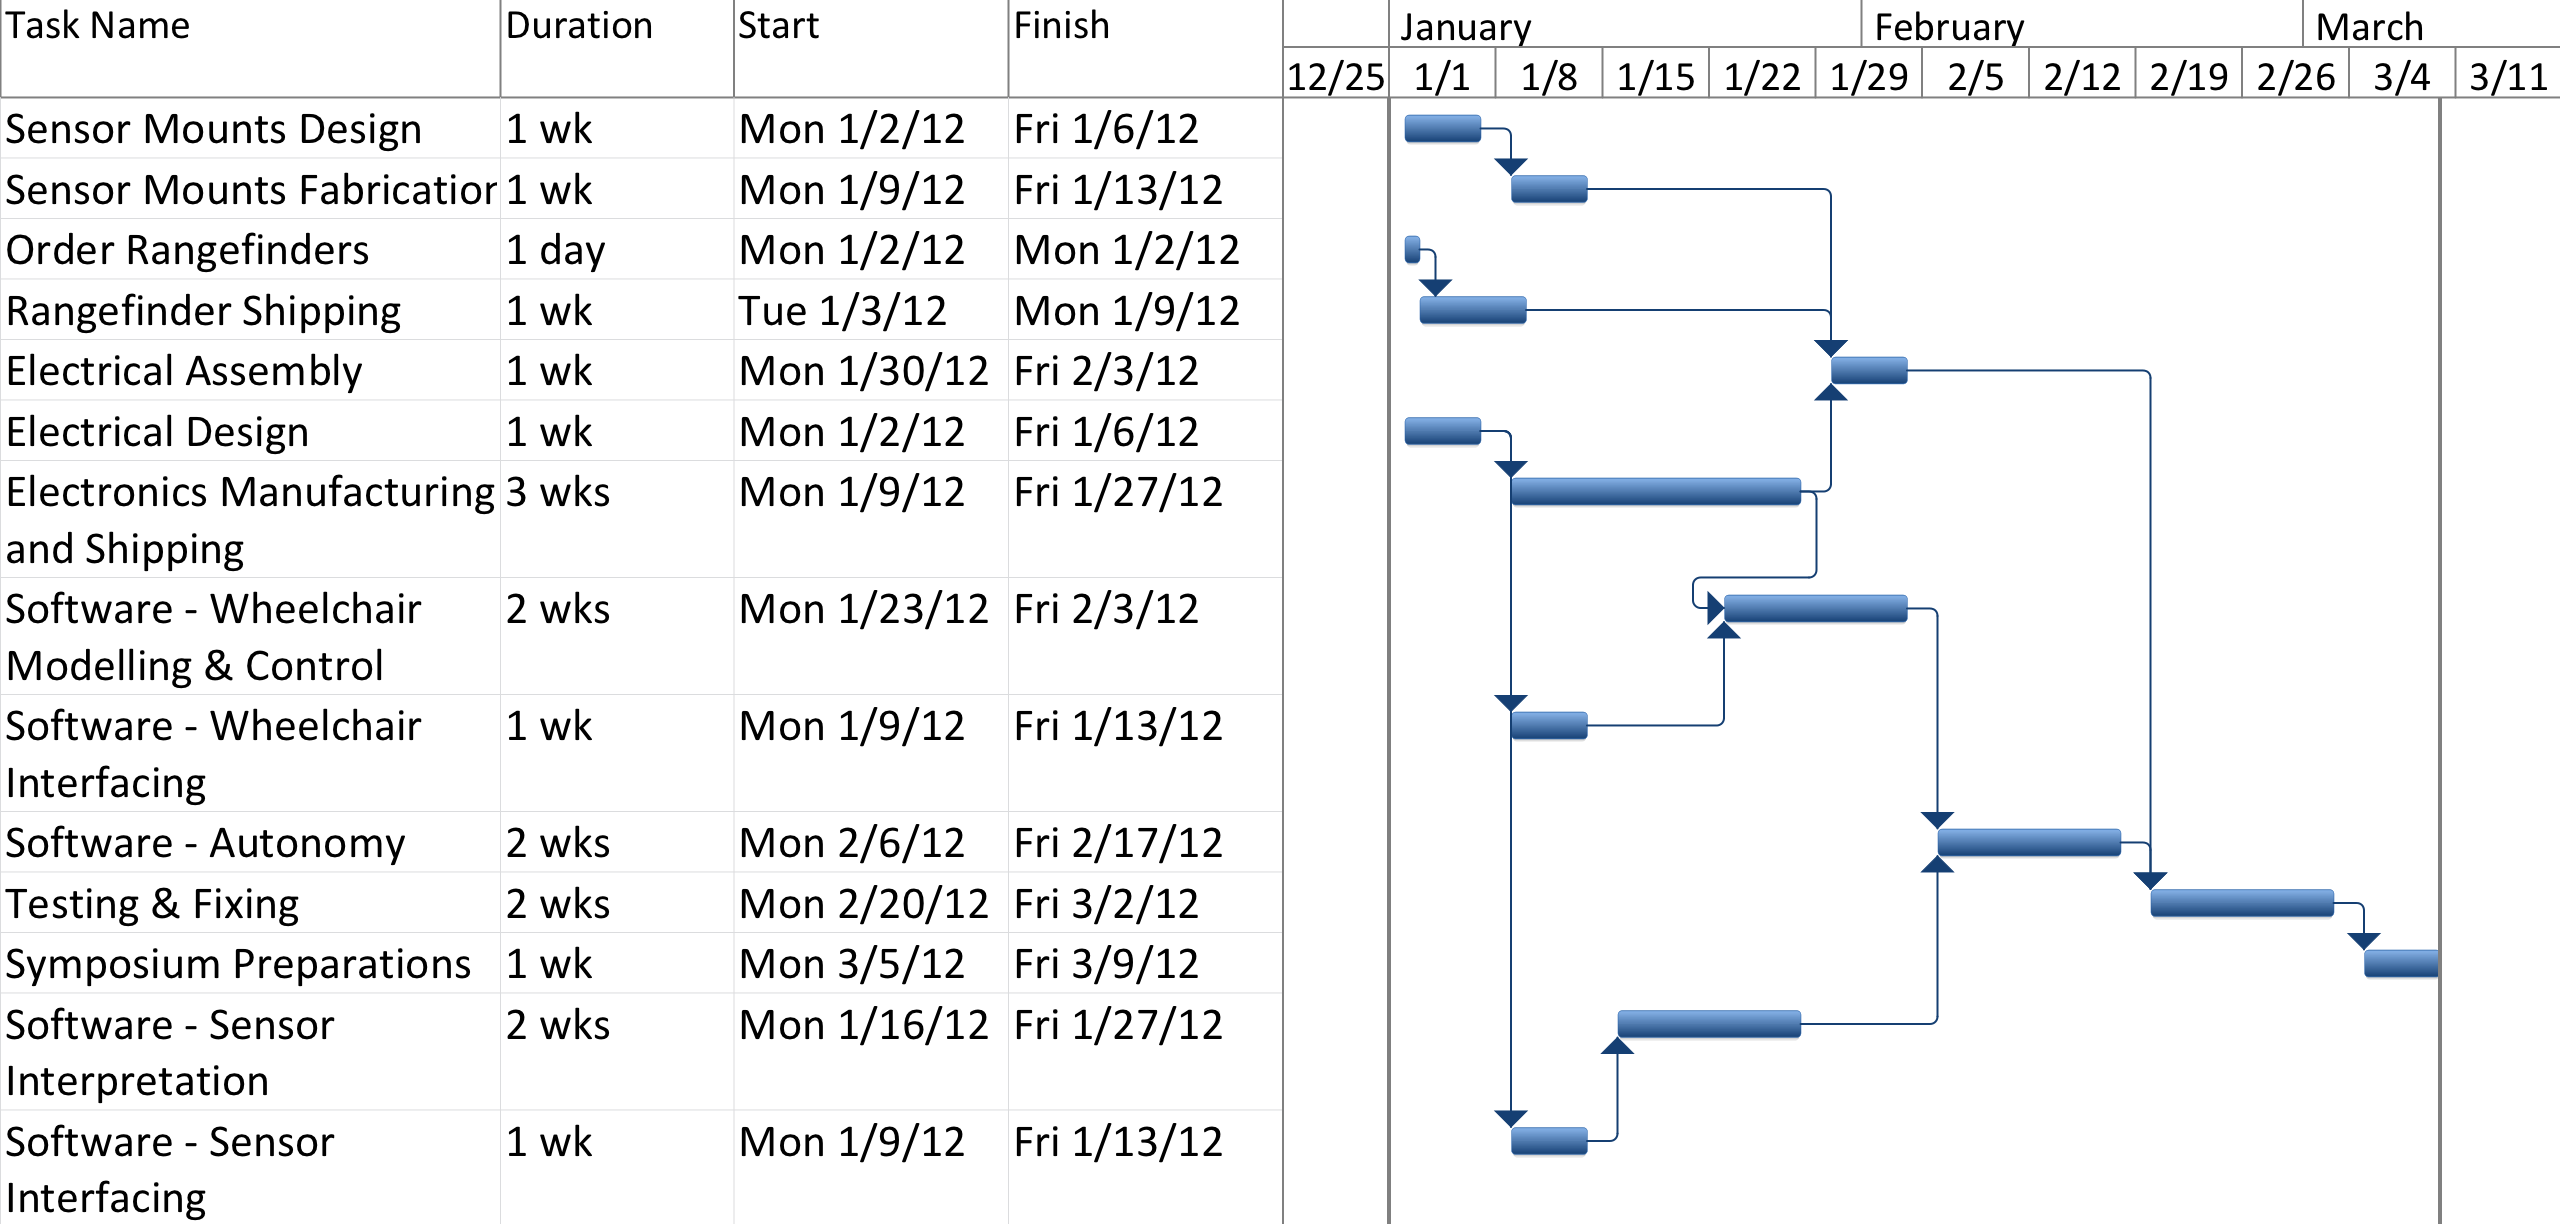
\includegraphics[scale=0.6]{gantt.png}
 \caption{Production schedule for the prototype}
 \label{schedule}
\end{figure}

Figure \ref{schedule} shows the prototype production gantt chart.  It may be seen that the prototype is expected to be completed about a week before the March symposium date.  The timeline is dominated by electrical and software tasks; if possible, it would be especially advantageous to begin electrical design work early.

\section{Bill of Materials}
\vspace{0.5cm}
\begin{figure}[h]
\centering
\begin{tabular}{|l|c|c|c|}
\hline
Part & Count & Cost (CAD) & Total (CAD) \\
\hline
Xbox Kinect & 1 & 150 & 150 \\
\hline
Xbox Kinect Mount & 1& 15 & 15 \\
Sonar Sensor & 4 & 30 & 120 \\
\hline
Sheet Metal & 1 & 12 & 12 \\
\hline
Spacers & 8 & 0.25 & 2 \\
\hline
PCB \& Components & 1 & 150 & 150 \\
\hline
Basic Netbook & 1 & 250 & 350 \\
\hline
\hline
Total&&&789\\
\hline
\end{tabular}
\caption{Bill of Materials}
\label{tab:BOM}
\end{figure}

Note that figure \ref{tab:BOM} shows the expected cost for the prototype system.  It is expected that, in production, economies of scale will reduce the unit cost to below the target price of \$500.

\chapter{Conclusions and Recommendations}
%TODO(?)

\chapter*{Appendix A}
\addcontentsline{toc}{chapter}{Appendix A - Patents}
%TODO(jordan)

\begin{thebibliography}{9}
 \addcontentsline{toc}{chapter}{Bibliography}

 % NB: cite these with \cite{item}

 \bibitem{lv-ez0}
   \emph{LV-EZ0 Datasheet}, MaxBotix Inc, 2011
 \bibitem{lv-ez4}
   \emph{LV-EZ4 Datasheet}, MaxBotix Inc, 2011
 \bibitem{kinect_prec}
  L. Yiping. “openni\_kinect/kinect\_accuracy” Internet: http://www.ros.org/wiki/openni\_kinect/kinect\_accuracy, Jun. 27, 2011.
 \bibitem{kinect_power }
  M. Wise. “Adding a Kinect to an iRobot Create.” Internet: http://www.ros.org/wiki/kinect/Tutorials/Adding\%20a\%20Kinect\%20to\%20an\%20iRobot\%20Create, May 2, 2011.
 \bibitem{patent:power_wheelchair}
  G. Griggs, T. Dutta, G. Fernie. “Powered Wheelchair.” U.S. Patent 2010/0082182A1, Apr. 1, 2010.
 \bibitem{patent:wheelchair_method}
  T. Smithers, U. Urriticoechea, U. Campos. “Wheelchair and Method for Correcting the Guidance of a Wheelchair.” U.S. Paten 2011/0130940A1, Jun. 2, 2011.
 \bibitem{patent:computer_controlled}
  L. Fehr, S. Skaar, G. Del Castillo. “Computer Controlled Power Wheelchair Navigation System.” U.S. Patent 2008/7383107B2, Jun. 3, 2008.
 \bibitem{MSP430_USB}
  A. Dannenberg. (2006, October). MSP430 Connectivity Using TUSB3410. Available: http://www.ti.com/lit/an/slaa276a/slaa276a.pdf
 \bibitem{primesense}
  "Our Full 3D Sensing Solution." Internet: http://www.primesense.com/en/technology/115-the-primesense-3d-sensing-solution, 2011.
 \bibitem{OpenNI}
  Insert generic reference to OpenNI website or package.
 \bibitem{ROS}
  Insert generic reference to ROS website or package.
 \bibitem{wheelchair_data}
  Invacare. "Nutron R51LXP. Invacare Product Catalogue." Internet: http://www.invacare.ca/cgi-bin/imhqprd/inv\_catalog/prod\_cat\_detail.jsp?s=0\&prodID=R51LXP\&catOID=-536887496, Jan. 2011.
 \bibitem{NASA}
  NASA. "NASA-STD-3000. Anthropometry and Biomechanics." Internet: http://msis.jsc.nasa.gov/sections/section03.htm, Jul. 1995.
 \bibitem{point_clouds}
  Insert generic reference to Point Cloud Library.
\end{thebibliography}


\end{document}